% Professional TikZ Figures for Bio-Adaptive Haptic Coaching
% Compilable with: pdflatex bioctl_tikz_figures.tex
% Usage: % Professional TikZ Figures for Bio-Adaptive Haptic Coaching
% Compilable with: pdflatex bioctl_tikz_figures.tex
% Usage: % Professional TikZ Figures for Bio-Adaptive Haptic Coaching
% Compilable with: pdflatex bioctl_tikz_figures.tex
% Usage: % Professional TikZ Figures for Bio-Adaptive Haptic Coaching
% Compilable with: pdflatex bioctl_tikz_figures.tex
% Usage: \input{bioctl_tikz_figures.tex} in your main document

\documentclass[12pt,border=5pt]{standalone}
\usepackage{tikz}
\usepackage{amsmath}
\usepackage{amssymb}

\usetikzlibrary{shapes,arrows,positioning,calc,fit,decorations.pathmorphing}

% Color scheme
\definecolor{pomdpblue}{RGB}{41,128,185}
\definecolor{rewardgreen}{RGB}{46,204,113}
\definecolor{hapticsred}{RGB}{231,76,60}
\definecolor{biomarkerviolet}{RGB}{155,89,182}
\definecolor{lightblue}{RGB}{174,194,224}
\definecolor{lightgreen}{RGB}{154,235,206}

% ============================================================================
% FIGURE 1: POMDP STRUCTURE WITH BIOMETRIC STATE
% ============================================================================

\begin{document}

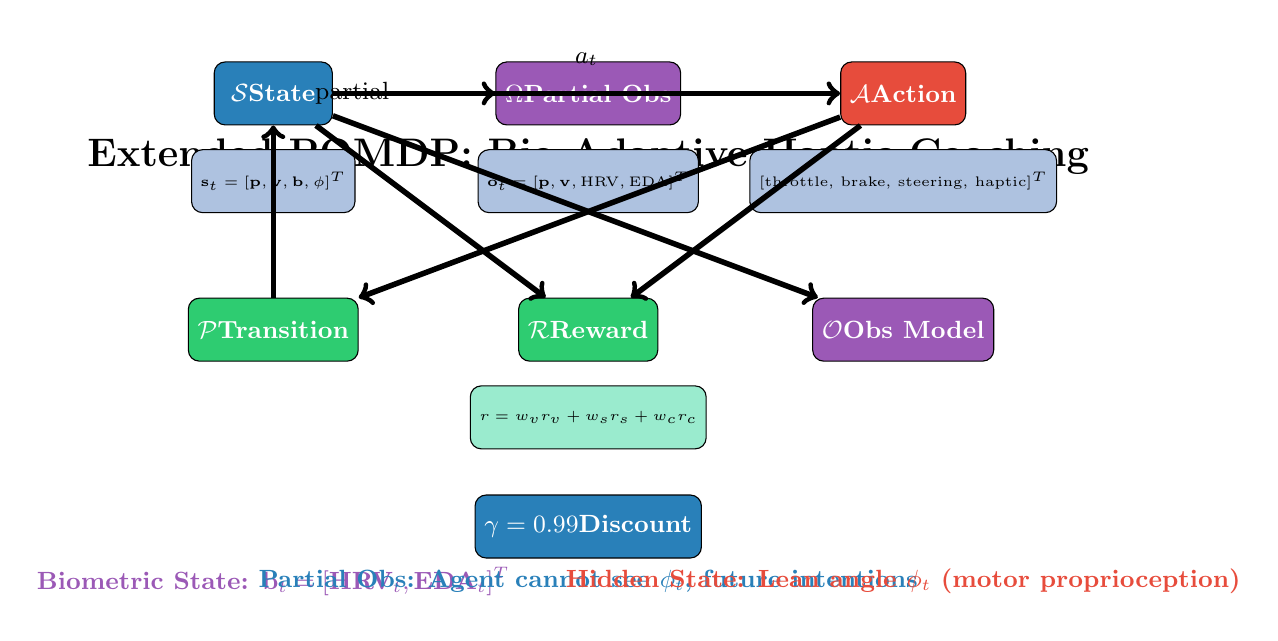
\begin{tikzpicture}[
    node distance=2.5cm,
    every node/.style={draw,rounded corners,minimum width=1.5cm,minimum height=0.8cm,font=\small\bfseries}
]

% Title
\node[draw=none,font=\Large\bfseries] at (6,-0.8) {Extended POMDP: Bio-Adaptive Haptic Coaching};

% State space
\node[fill=pomdpblue,text=white] (state) at (2,0) {$\mathcal{S}$\\State};
\node[fill=lightblue,text=black,below=0.3cm of state,draw,font=\tiny,rounded corners] {$\mathbf{s}_t = [\mathbf{p}, \mathbf{v}, \mathbf{b}, \phi]^T$};

% Observation space (partial)
\node[fill=biomarkerviolet,text=white] (obs) at (6,0) {$\Omega$\\Partial Obs};
\node[fill=lightblue,text=black,below=0.3cm of obs,draw,font=\tiny,rounded corners] {$\mathbf{o}_t = [\mathbf{p}, \mathbf{v}, \text{HRV}, \text{EDA}]^T$};

% Action space
\node[fill=hapticsred,text=white] (action) at (10,0) {$\mathcal{A}$\\Action};
\node[fill=lightblue,text=black,below=0.3cm of action,draw,font=\tiny,rounded corners] {$[\text{throttle, brake, steering, haptic}]^T$};

% Transition model
\node[fill=rewardgreen,text=white] (trans) at (2,-3) {$\mathcal{P}$\\Transition};

% Reward function
\node[fill=rewardgreen,text=white] (reward) at (6,-3) {$\mathcal{R}$\\Reward};
\node[fill=lightgreen,text=black,below=0.3cm of reward,draw,font=\tiny,rounded corners] {$r = w_v r_v + w_s r_s + w_c r_c$};

% Observation model
\node[fill=biomarkerviolet,text=white] (obsmodel) at (10,-3) {$\mathcal{O}$\\Obs Model};

% Discount factor
\node[fill=pomdpblue,text=white] (discount) at (6,-5.5) {$\gamma = 0.99$\\Discount};

% Connections
\draw[->,line width=2pt] (state) -- node[above,draw=none,font=\small] {$a_t$} (action);
\draw[->,line width=2pt] (action) -- (trans);
\draw[->,line width=2pt] (trans) -- (state);
\draw[->,line width=2pt] (state) -- (reward);
\draw[->,line width=2pt] (action) -- (reward);
\draw[->,line width=2pt] (state) -- node[left,draw=none,font=\small] {partial} (obs);
\draw[->,line width=2pt] (state) -- (obsmodel);

% Biometric component highlight
\node[draw=none,font=\small\bfseries,text=biomarkerviolet] at (2,-6.2) {\textbf{Biometric State:} $\mathbf{b}_t = [\text{HRV}_t, \text{EDA}_t]^T$};
\node[draw=none,font=\small\bfseries,text=pomdpblue] at (6,-6.2) {\textbf{Partial Obs:} Agent cannot see $\phi_t$, future intentions};
\node[draw=none,font=\small\bfseries,text=hapticsred] at (10,-6.2) {\textbf{Hidden State:} Lean angle $\phi_t$ (motor proprioception)};

\end{tikzpicture}

\pagebreak

% ============================================================================
% FIGURE 2: MULTI-OBJECTIVE REWARD SCALARIZATION
% ============================================================================

\begin{tikzpicture}

% Title
\node[draw=none,font=\Large\bfseries] at (7,-0.5) {Multi-Objective Reward Scalarization};

% Velocity reward
\begin{scope}[shift=(0,0)]
\node[fill=rewardgreen,text=white,font=\small\bfseries] at (2,2) {$r_v$ (Velocity)};
\draw[thick, rewardgreen] (0.5,0) -- (1,0.3) -- (2,0.8) -- (3,1.2) -- (3.5,1.5);
\draw[dashed,gray] (0,0) -- (4,0) -- (4,2) -- (0,2) -- (0,0);
\node[draw=none,font=\tiny] at (2,-0.4) {Speed $\rightarrow$};
\node[draw=none,font=\tiny] at (-0.5,1) {Reward};
\node[draw=none,font=\tiny] at (2,-0.8) {Weight: $w_v = 0.50$};
\end{scope}

% Safety reward
\begin{scope}[shift=(5,0)]
\node[fill=rewardgreen,text=white,font=\small\bfseries] at (2,2) {$r_s$ (Safety)};
\draw[thick, rewardgreen] (0.5,0.05) -- (1,0.3) -- (2,0.8) -- (3,1.3) -- (3.5,1.45);
\draw[dashed,gray] (0,0) -- (4,0) -- (4,2) -- (0,2) -- (0,0);
\node[draw=none,font=\tiny] at (2,-0.4) {Distance to obstacle};
\node[draw=none,font=\tiny] at (-0.5,1) {Reward};
\node[draw=none,font=\tiny] at (2,-0.8) {Weight: $w_s = 0.35$};
\end{scope}

% Cognitive Load reward
\begin{scope}[shift=(10,0)]
\node[fill=biomarkerviolet,text=white,font=\small\bfseries] at (2,2) {$r_c$ (Cog Load)};
% Safe zone
\draw[thick, biomarkerviolet] (0.5,1.5) -- (1.8,1.5);
% Risk zone
\draw[thick, biomarkerviolet] (1.8,1.5) -- (3,0.3);
% Panic zone
\draw[thick, biomarkerviolet, dashed] (3,0.3) -- (3.5,-0.5);
\draw[dashed,gray] (0,0) -- (4,0) -- (4,2) -- (0,2) -- (0,0);
\node[draw=none,font=\tiny,text=green] at (1.2,1.8) {RMSSD>50};
\node[draw=none,font=\tiny,text=orange] at (2.5,0.8) {10-50};
\node[draw=none,font=\tiny,text=red] at (3.2,-0.2) {<10};
\node[draw=none,font=\tiny] at (-0.5,1) {Reward};
\node[draw=none,font=\tiny] at (2,-0.8) {Weight: $w_c = 0.15$};
\end{scope}

% Weighted combination
\node[draw=none,font=\normalsize\bfseries,fill=yellow!20,inner sep=10pt] at (7,-2.5) {$r_t = 0.50 \cdot r_v + 0.35 \cdot r_s + 0.15 \cdot r_c$};

\node[draw=none,font=\tiny,text=darkgray,inner sep=5pt] at (7,-3.3) {Objective function: $J(\pi) = \mathbb{E}[\sum_t \gamma^t r_t]$ maximized by policy gradient};

\end{tikzpicture}

\pagebreak

% ============================================================================
% FIGURE 3: BIO-SUPERVISOR ARCHITECTURE
% ============================================================================

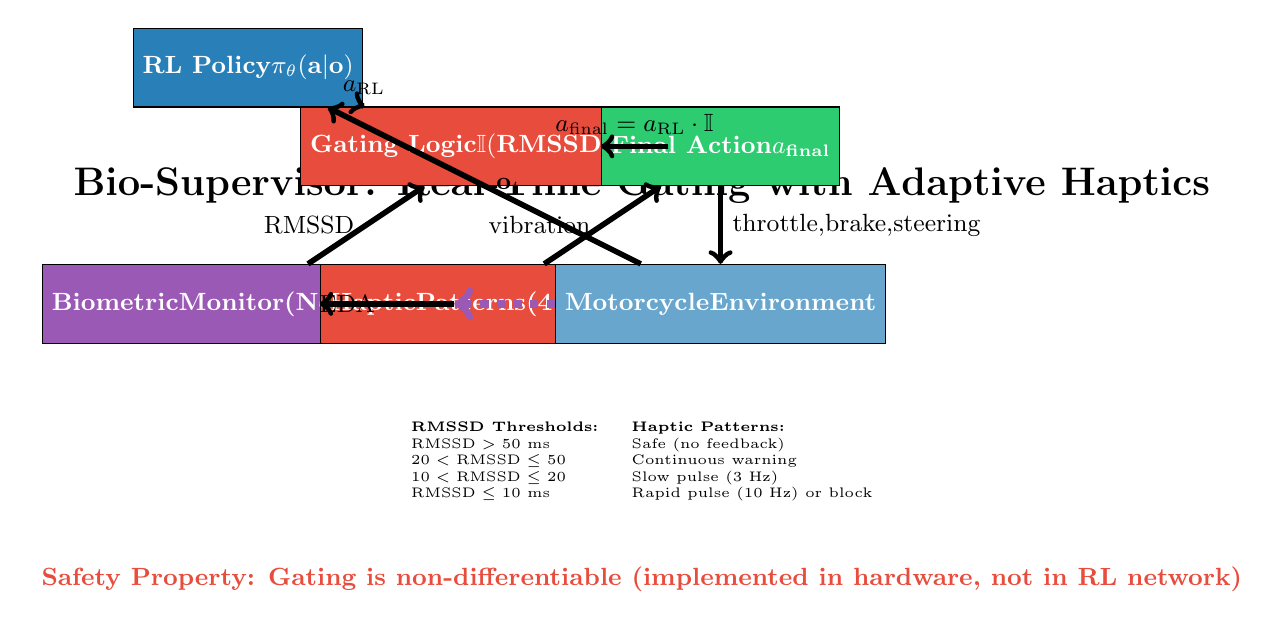
\begin{tikzpicture}[
    node distance=2cm,
]

% Title
\node[draw=none,font=\Large\bfseries] at (7,-0.5) {Bio-Supervisor: Real-Time Gating with Adaptive Haptics};

% RL Policy
\node[draw,fill=pomdpblue,text=white,font=\small\bfseries,minimum width=2.5cm,minimum height=1cm] (rl) at (2,1) {RL Policy\\$\pi_\theta(\mathbf{a}|\mathbf{o})$};

% Biometric Monitor
\node[draw,fill=biomarkerviolet,text=white,font=\small\bfseries,minimum width=2.5cm,minimum height=1cm] (bio) at (2,-2) {Biometric\\Monitor\\(NeuroKit2)};

% Gating logic
\node[draw,fill=hapticsred,text=white,font=\small\bfseries,minimum width=2.5cm,minimum height=1cm] (gating) at (5,0) {Gating Logic\\$\mathbb{I}(\text{RMSSD} > \theta)$};

% Haptic feedback
\node[draw,fill=hapticsred,text=white,font=\small\bfseries,minimum width=2.5cm,minimum height=1cm] (haptic) at (5,-2) {Haptic\\Patterns\\(4-stage)};

% Final action
\node[draw,fill=rewardgreen,text=white,font=\small\bfseries,minimum width=2.5cm,minimum height=1cm] (action) at (8,0) {Final Action\\$a_{\text{final}}$};

% Motorcycle environment
\node[draw,fill=pomdpblue!70,text=white,font=\small\bfseries,minimum width=2.5cm,minimum height=1cm] (env) at (8,-2) {Motorcycle\\Environment};

% Connections
\draw[->,line width=2pt] (rl) -- node[above,draw=none,font=\small] {$a_{\text{RL}}$} (gating);
\draw[->,line width=2pt] (gating) -- node[above,draw=none,font=\small] {$a_{\text{final}} = a_{\text{RL}} \cdot \mathbb{I}$} (action);

\draw[->,line width=2pt] (bio) -- node[left,draw=none,font=\small] {RMSSD} (gating);
\draw[->,line width=2pt] (bio) -- node[left,draw=none,font=\small] {EDA} (haptic);
\draw[->,line width=2pt] (haptic) -- node[left,draw=none,font=\small] {vibration} (action);

\draw[->,line width=2pt] (action) -- node[right,draw=none,font=\small] {throttle,\\brake,\\steering} (env);
\draw[->,line width=3pt,dashed,biomarkerviolet] (env) -- (bio);
\draw[->,line width=2pt] (env) -- node[right,draw=none,font=\small] {$\mathbf{o}_t$} (rl);

% Legend box
\node[draw=none,font=\tiny,inner sep=5pt] at (7,-4) {
\begin{tabular}{ll}
\textbf{RMSSD Thresholds:} & \textbf{Haptic Patterns:} \\
$\text{RMSSD} > 50$ ms & Safe (no feedback) \\
$20 < \text{RMSSD} \leq 50$ & Continuous warning \\
$10 < \text{RMSSD} \leq 20$ & Slow pulse (3 Hz) \\
$\text{RMSSD} \leq 10$ ms & Rapid pulse (10 Hz) or block \\
\end{tabular}
};

\node[draw=none,font=\small\bfseries,text=hapticsred,inner sep=5pt] at (7,-5.5) {\textbf{Safety Property:} Gating is non-differentiable (implemented in hardware, not in RL network)};

\end{tikzpicture}

\pagebreak

% ============================================================================
% FIGURE 4: POLICY ARCHITECTURE WITH BIOMETRIC FUSION
% ============================================================================

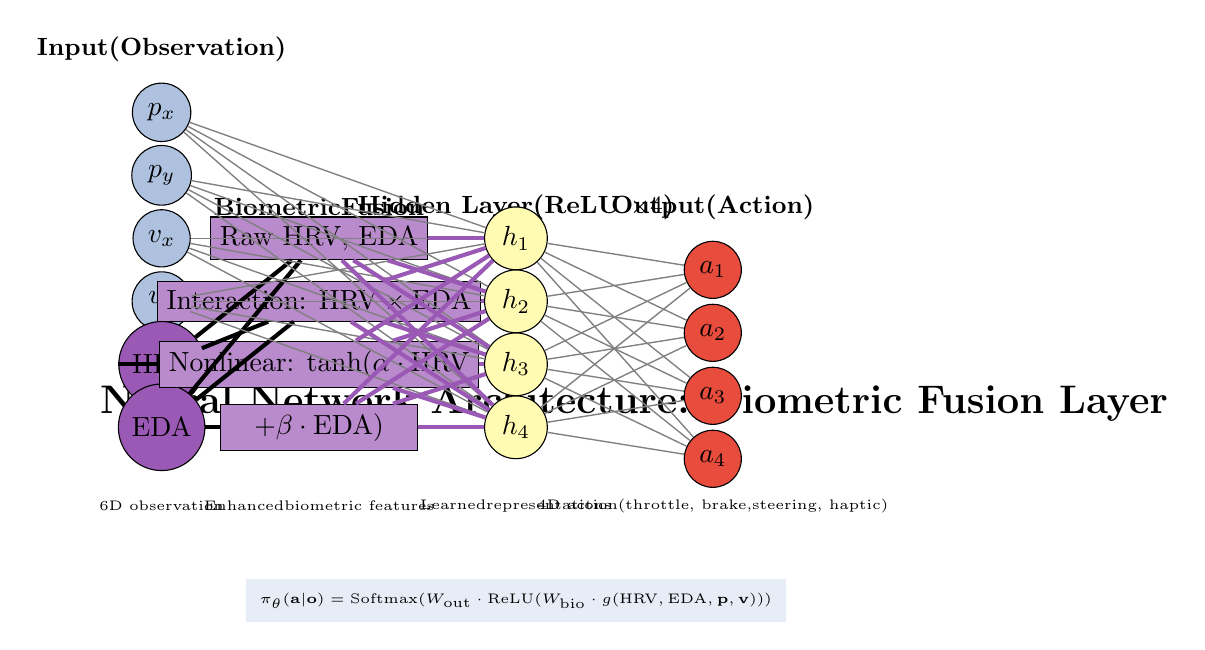
\begin{tikzpicture}[
    node distance=1.5cm,
]

% Title
\node[draw=none,font=\Large\bfseries] at (7,-0.5) {Neural Network Architecture: Biometric Fusion Layer};

% Input layer
\node[draw=none,font=\small\bfseries] at (1,4) {Input\\(Observation)};

\node[draw,fill=lightblue,circle,minimum size=0.6cm] (p1) at (1,3.2) {$p_x$};
\node[draw,fill=lightblue,circle,minimum size=0.6cm] (p2) at (1,2.4) {$p_y$};
\node[draw,fill=lightblue,circle,minimum size=0.6cm] (v1) at (1,1.6) {$v_x$};
\node[draw,fill=lightblue,circle,minimum size=0.6cm] (v2) at (1,0.8) {$v_y$};
\node[draw,fill=biomarkerviolet,circle,minimum size=0.6cm] (hrv) at (1,0) {HRV};
\node[draw,fill=biomarkerviolet,circle,minimum size=0.6cm] (eda) at (1,-0.8) {EDA};

% Biometric fusion layer
\node[draw=none,font=\small\bfseries] at (3,2) {Biometric\\Fusion};

\node[draw,fill=biomarkerviolet!70,rectangle,minimum width=2.5cm,minimum height=0.5cm] (fusion1) at (3,1.6) {Raw HRV, EDA};
\node[draw,fill=biomarkerviolet!70,rectangle,minimum width=2.5cm,minimum height=0.5cm] (fusion2) at (3,0.8) {Interaction: $\text{HRV} \times \text{EDA}$};
\node[draw,fill=biomarkerviolet!70,rectangle,minimum width=2.5cm,minimum height=0.5cm] (fusion3) at (3,0) {Nonlinear: $\tanh(\alpha\cdot\text{HRV}$};
\node[draw,fill=biomarkerviolet!70,rectangle,minimum width=2.5cm,minimum height=0.5cm] (fusion4) at (3,-0.8) {$+\beta\cdot\text{EDA})$};

% Hidden layer
\node[draw=none,font=\small\bfseries] at (5.5,2) {Hidden Layer\\(ReLU $\times 4$)};

\node[draw,fill=yellow!30,circle,minimum size=0.6cm] (h1) at (5.5,1.6) {$h_1$};
\node[draw,fill=yellow!30,circle,minimum size=0.6cm] (h2) at (5.5,0.8) {$h_2$};
\node[draw,fill=yellow!30,circle,minimum size=0.6cm] (h3) at (5.5,0) {$h_3$};
\node[draw,fill=yellow!30,circle,minimum size=0.6cm] (h4) at (5.5,-0.8) {$h_4$};

% Output layer
\node[draw=none,font=\small\bfseries] at (8,2) {Output\\(Action)};

\node[draw,fill=hapticsred,circle,minimum size=0.6cm] (a1) at (8,1.2) {$a_1$};
\node[draw,fill=hapticsred,circle,minimum size=0.6cm] (a2) at (8,0.4) {$a_2$};
\node[draw,fill=hapticsred,circle,minimum size=0.6cm] (a3) at (8,-0.4) {$a_3$};
\node[draw,fill=hapticsred,circle,minimum size=0.6cm] (a4) at (8,-1.2) {$a_4$};

% Connections from input to fusion
\draw[-,line width=1.5pt] (hrv) -- (fusion1);
\draw[-,line width=1.5pt] (eda) -- (fusion1);
\draw[-,line width=1.5pt] (hrv) -- (fusion2);
\draw[-,line width=1.5pt] (eda) -- (fusion2);
\draw[-,line width=1.5pt] (hrv) -- (fusion3);
\draw[-,line width=1.5pt] (eda) -- (fusion4);

% Connections from position/velocity to hidden
\foreach \s in {p1,p2,v1,v2}
    \foreach \h in {h1,h2,h3,h4}
        \draw[-,line width=0.5pt,gray] (\s) -- (\h);

% Connections from fusion to hidden
\foreach \f in {fusion1,fusion2,fusion3,fusion4}
    \foreach \h in {h1,h2,h3,h4}
        \draw[-,line width=1.5pt,biomarkerviolet] (\f) -- (\h);

% Connections from hidden to output
\foreach \h in {h1,h2,h3,h4}
    \foreach \a in {a1,a2,a3,a4}
        \draw[-,line width=0.5pt,gray] (\h) -- (\a);

% Labels
\node[draw=none,font=\tiny] at (1,-1.8) {6D observation};
\node[draw=none,font=\tiny] at (3,-1.8) {Enhanced\\biometric features};
\node[draw=none,font=\tiny] at (5.5,-1.8) {Learned\\representations};
\node[draw=none,font=\tiny] at (8,-1.8) {4D action\\(throttle, brake,\\steering, haptic)};

% Formula box
\node[draw=none,font=\tiny,inner sep=5pt,fill=lightblue!30] at (5.5,-3) {
$\pi_\theta(\mathbf{a}|\mathbf{o}) = \text{Softmax}(W_{\text{out}} \cdot \text{ReLU}(W_{\text{bio}} \cdot g(\text{HRV}, \text{EDA}, \mathbf{p}, \mathbf{v})))$
};

\end{tikzpicture}

\pagebreak

% ============================================================================
% FIGURE 5: RMSSD-BASED COGNITIVE LOAD REWARD
% ============================================================================

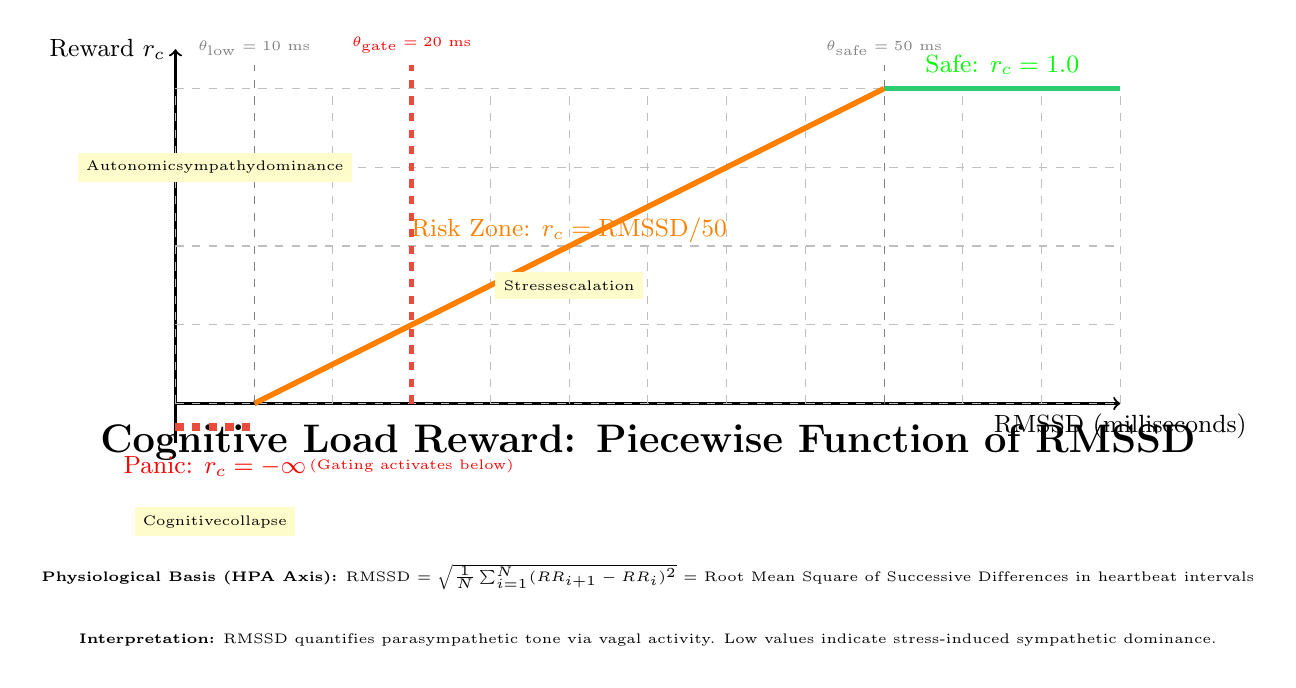
\begin{tikzpicture}

% Title
\node[draw=none,font=\Large\bfseries] at (7,-0.5) {Cognitive Load Reward: Piecewise Function of RMSSD};

% Axes
\draw[thick,->] (1,0) -- (13,0) node[below,font=\small] {RMSSD (milliseconds)};
\draw[thick,->] (1,-0.5) -- (1,4.5) node[left,font=\small] {Reward $r_c$};

% Grid
\draw[dashed,gray!50] (1,0) grid[step=1] (13,4);

% Function pieces
% Safe zone (RMSSD >= 50)
\draw[thick, rewardgreen, line width=2pt] (10,4) -- (13,4);
\node[draw=none,font=\small,text=green] at (11.5,4.3) {Safe: $r_c = 1.0$};

% Linear zone (10 < RMSSD < 50)
\draw[thick, orange, line width=2pt] (2,0) -- (10,4);
\node[draw=none,font=\small,text=orange] at (6,2.2) {Risk Zone: $r_c = \text{RMSSD}/50$};

% Panic zone (RMSSD <= 10)
\draw[thick, hapticsred, line width=3pt, dashed] (1,-0.3) -- (2,-0.3);
\node[draw=none,font=\small,text=red] at (1.5,-0.8) {Panic: $r_c = -\infty$};

% Threshold lines
\draw[dashed, gray] (2,0) -- (2,4.3) node[above,font=\tiny] {$\theta_{\text{low}} = 10$ ms};
\draw[dashed, gray] (10,0) -- (10,4.3) node[above,font=\tiny] {$\theta_{\text{safe}} = 50$ ms};

% Gating threshold
\draw[dashed, hapticsred, line width=2pt] (4,0) -- (4,4.3) node[above,font=\tiny,text=red] {$\theta_{\text{gate}} = 20$ ms};
\node[draw=none,font=\tiny,text=red] at (4,-0.8) {(Gating activates below)};

% Annotations
\node[draw=none,font=\tiny,inner sep=3pt,fill=yellow!20] at (1.5,3) {Autonomic\\sympathy\\dominance};
\node[draw=none,font=\tiny,inner sep=3pt,fill=yellow!20] at (6,1.5) {Stress\\escalation};
\node[draw=none,font=\tiny,inner sep=3pt,fill=yellow!20] at (1.5,-1.5) {Cognitive\\collapse};

% Legend
\node[draw=none,font=\tiny,inner sep=5pt] at (7,-2.2) {
\textbf{Physiological Basis (HPA Axis):}
RMSSD = $\sqrt{\frac{1}{N}\sum_{i=1}^N (RR_{i+1} - RR_i)^2}$ = Root Mean Square of Successive Differences in heartbeat intervals
};

\node[draw=none,font=\tiny,inner sep=5pt] at (7,-3) {
\textbf{Interpretation:} RMSSD quantifies parasympathetic tone via vagal activity. Low values indicate stress-induced sympathetic dominance.
};

\end{tikzpicture}

\pagebreak

% ============================================================================
% FIGURE 6: STATE SPACE DIMENSIONALITY
% ============================================================================

\begin{tikzpicture}

% Title
\node[draw=none,font=\Large\bfseries] at (7,-0.5) {State Space: 7D Hidden vs 6D Observed};

% Hidden state box
\node[draw,fill=pomdpblue,text=white,font=\small\bfseries,minimum width=4cm,minimum height=3cm] (hidden) at (2.5,1.5) {
\begin{tabular}{c}
\textbf{Hidden State} $\mathbf{s}_t \in \mathbb{R}^7$ \\
\\
$p_x$ (position X) \\
$p_y$ (position Y) \\
$v_x$ (velocity X) \\
$v_y$ (velocity Y) \\
HRV (Heart Rate Var.) \\
EDA (Electro. Dermal) \\
$\phi$ (lean angle) \textcolor{red}{???}
\end{tabular}
};

% Observation box
\node[draw,fill=biomarkerviolet,text=white,font=\small\bfseries,minimum width=4cm,minimum height=2.5cm] (obs) at (7.5,1.5) {
\begin{tabular}{c}
\textbf{Observed} $\mathbf{o}_t \in \mathbb{R}^6$ \\
\\
$p_x$ (position X) \\
$p_y$ (position Y) \\
$v_x$ (velocity X) \\
$v_y$ (velocity Y) \\
HRV (Heart Rate Var.) \\
EDA (Electro. Dermal)
\end{tabular}
};

% Arrow showing loss of information
\draw[->,line width=3pt,red] (4.8,2) -- (5.7,2) node[above,draw=none,font=\small,text=red] {Partial\\Observability};

% Explanation
\node[draw=none,font=\small,text=darkred,inner sep=5pt,fill=red!10] at (5,0.3) {
Motorcycle lean angle $\phi$ is \textbf{hidden} from agent \\
(proprioceptive sensing not available in coaching context)
};

% Agent belief
\node[draw,fill=rewardgreen!70,text=white,font=\small\bfseries,minimum width=3cm,minimum height=1.5cm] (belief) at (5,-2.5) {
\begin{tabular}{c}
\textbf{Agent Belief} \\
State via Bayesian Filter \\
$b_t(s_t) = \frac{\mathcal{O}(o_t|s_t) P(s_t|s_{t-1},a_{t-1}) b_{t-1}(s_{t-1})}{\mathcal{O}(o_t)}$
\end{tabular}
};

\draw[->,line width=2pt] (2.5,0.2) -- (belief);
\draw[->,line width=2pt] (7.5,0.2) -- (belief);

\end{tikzpicture}

\pagebreak

% ============================================================================
% FIGURE 7: TRAINING ALGORITHM FLOWCHART
% ============================================================================

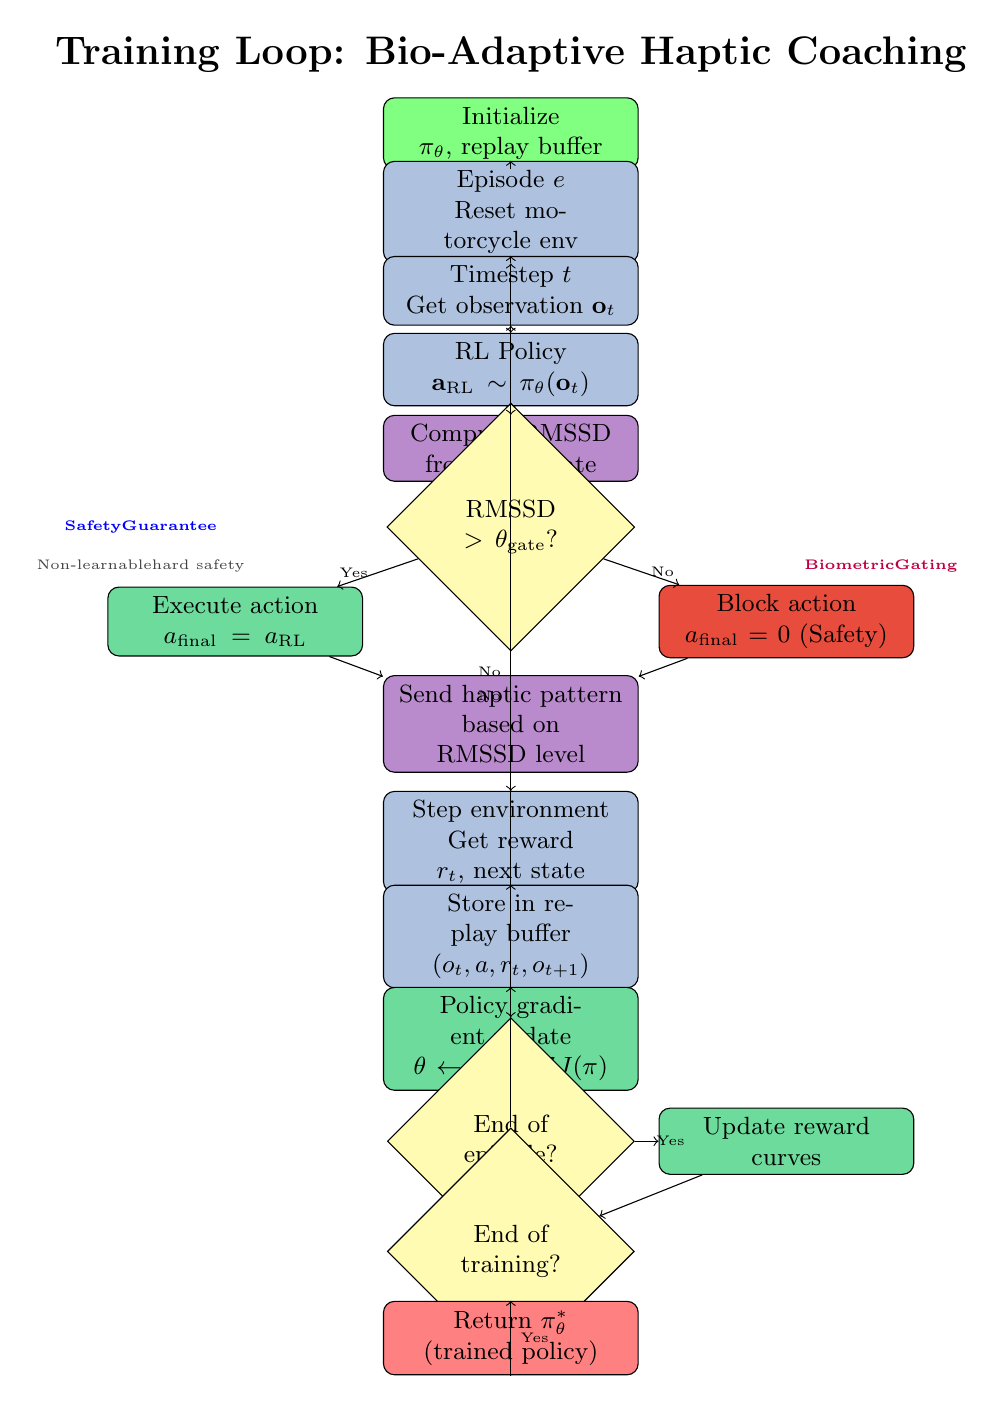
\begin{tikzpicture}[
    node distance=1.8cm,
    block/.style={draw, fill=lightblue, text width=3cm, text centered, rounded corners, minimum height=0.8cm, font=\small},
    decision/.style={diamond, draw, fill=yellow!30, text width=2cm, text centered, minimum height=1cm, font=\small},
    action/.style={draw, fill=rewardgreen!70, text width=3cm, text centered, rounded corners, minimum height=0.8cm, font=\small},
    bioaction/.style={draw, fill=biomarkerviolet!70, text width=3cm, text centered, rounded corners, minimum height=0.8cm, font=\small}
]

% Title
\node[draw=none,font=\Large\bfseries] at (5,9) {Training Loop: Bio-Adaptive Haptic Coaching};

% Start
\node[block,fill=green!50] (start) at (5,8) {Initialize\\$\pi_\theta$, replay buffer};

% Episode
\node[block] (episode) at (5,7) {Episode $e$\\Reset motorcycle env};

% Timestep
\node[block] (timestep) at (5,6) {Timestep $t$\\Get observation $\mathbf{o}_t$};

% Action selection
\node[block] (action) at (5,5) {RL Policy\\$\mathbf{a}_{\text{RL}} \sim \pi_\theta(\mathbf{o}_t)$};

% Compute RMSSD
\node[bioaction] (rmssd) at (5,4) {Compute RMSSD\\from heart rate};

% Gating decision
\node[decision] (gate) at (5,3) {RMSSD\\$> \theta_{\text{gate}}$?};

% Gating true
\node[action] (gate_true) at (1.5,1.8) {Execute action\\$a_{\text{final}} = a_{\text{RL}}$};

% Gating false
\node[action,fill=hapticsred] (gate_false) at (8.5,1.8) {Block action\\$a_{\text{final}} = 0$ (Safety)};

% Haptic feedback
\node[bioaction] (haptic) at (5,0.5) {Send haptic pattern\\based on RMSSD level};

% Step environment
\node[block] (step) at (5,-1) {Step environment\\Get reward $r_t$, next state};

% Store transition
\node[block] (store) at (5,-2.2) {Store in replay buffer\\$(o_t, a, r_t, o_{t+1})$};

% Update policy
\node[action] (update) at (5,-3.5) {Policy gradient update\\$\theta \leftarrow \theta + \alpha \nabla J(\pi)$};

% End of episode?
\node[decision] (eod) at (5,-4.8) {End of\\episode?};

% Update curves
\node[action] (curves) at (8.5,-4.8) {Update reward\\curves};

% End training?
\node[decision] (eot) at (5,-6.2) {End of\\training?};

% End
\node[block,fill=red!50] (end) at (5,-7.3) {Return $\pi_\theta^*$\\(trained policy)};

% Connections
\draw[->] (start) -- (episode);
\draw[->] (episode) -- (timestep);
\draw[->] (timestep) -- (action);
\draw[->] (action) -- (rmssd);
\draw[->] (rmssd) -- (gate);

\draw[->] (gate) -- node[left,draw=none,font=\tiny] {Yes} (gate_true);
\draw[->] (gate) -- node[right,draw=none,font=\tiny] {No} (gate_false);

\draw[->] (gate_true) -- (haptic);
\draw[->] (gate_false) -- (haptic);

\draw[->] (haptic) -- (step);
\draw[->] (step) -- (store);
\draw[->] (store) -- (update);

\draw[->] (update) -- (eod);
\draw[->] (eod) -- node[left,draw=none,font=\tiny] {No} (timestep);
\draw[->] (eod) -- node[right,draw=none,font=\tiny] {Yes} (curves);

\draw[->] (curves) -- (eot);
\draw[->] (eot) -- node[left,draw=none,font=\tiny] {No} (episode);
\draw[->] (eot) -- node[right,draw=none,font=\tiny] {Yes} (end);

% Side notes
\node[draw=none,font=\tiny,text=blue,inner sep=3pt] at (0.3,3) {\textbf{Safety\\Guarantee}};
\node[draw=none,font=\tiny,text=darkgray] at (0.3,2.5) {Non-learnable\\hard safety};

\node[draw=none,font=\tiny,text=purple,inner sep=3pt] at (9.7,2.5) {\textbf{Biometric\\Gating}};

\end{tikzpicture}

\end{document}
 in your main document

\documentclass[12pt,border=5pt]{standalone}
\usepackage{tikz}
\usepackage{amsmath}
\usepackage{amssymb}

\usetikzlibrary{shapes,arrows,positioning,calc,fit,decorations.pathmorphing}

% Color scheme
\definecolor{pomdpblue}{RGB}{41,128,185}
\definecolor{rewardgreen}{RGB}{46,204,113}
\definecolor{hapticsred}{RGB}{231,76,60}
\definecolor{biomarkerviolet}{RGB}{155,89,182}
\definecolor{lightblue}{RGB}{174,194,224}
\definecolor{lightgreen}{RGB}{154,235,206}

% ============================================================================
% FIGURE 1: POMDP STRUCTURE WITH BIOMETRIC STATE
% ============================================================================

\begin{document}

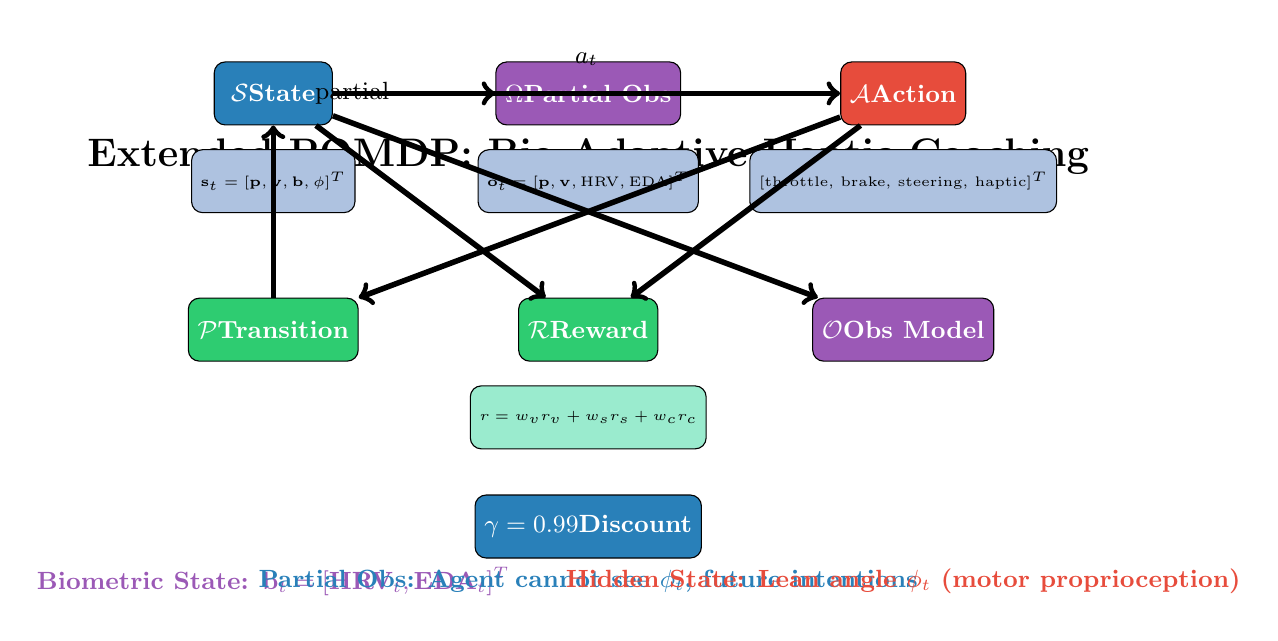
\begin{tikzpicture}[
    node distance=2.5cm,
    every node/.style={draw,rounded corners,minimum width=1.5cm,minimum height=0.8cm,font=\small\bfseries}
]

% Title
\node[draw=none,font=\Large\bfseries] at (6,-0.8) {Extended POMDP: Bio-Adaptive Haptic Coaching};

% State space
\node[fill=pomdpblue,text=white] (state) at (2,0) {$\mathcal{S}$\\State};
\node[fill=lightblue,text=black,below=0.3cm of state,draw,font=\tiny,rounded corners] {$\mathbf{s}_t = [\mathbf{p}, \mathbf{v}, \mathbf{b}, \phi]^T$};

% Observation space (partial)
\node[fill=biomarkerviolet,text=white] (obs) at (6,0) {$\Omega$\\Partial Obs};
\node[fill=lightblue,text=black,below=0.3cm of obs,draw,font=\tiny,rounded corners] {$\mathbf{o}_t = [\mathbf{p}, \mathbf{v}, \text{HRV}, \text{EDA}]^T$};

% Action space
\node[fill=hapticsred,text=white] (action) at (10,0) {$\mathcal{A}$\\Action};
\node[fill=lightblue,text=black,below=0.3cm of action,draw,font=\tiny,rounded corners] {$[\text{throttle, brake, steering, haptic}]^T$};

% Transition model
\node[fill=rewardgreen,text=white] (trans) at (2,-3) {$\mathcal{P}$\\Transition};

% Reward function
\node[fill=rewardgreen,text=white] (reward) at (6,-3) {$\mathcal{R}$\\Reward};
\node[fill=lightgreen,text=black,below=0.3cm of reward,draw,font=\tiny,rounded corners] {$r = w_v r_v + w_s r_s + w_c r_c$};

% Observation model
\node[fill=biomarkerviolet,text=white] (obsmodel) at (10,-3) {$\mathcal{O}$\\Obs Model};

% Discount factor
\node[fill=pomdpblue,text=white] (discount) at (6,-5.5) {$\gamma = 0.99$\\Discount};

% Connections
\draw[->,line width=2pt] (state) -- node[above,draw=none,font=\small] {$a_t$} (action);
\draw[->,line width=2pt] (action) -- (trans);
\draw[->,line width=2pt] (trans) -- (state);
\draw[->,line width=2pt] (state) -- (reward);
\draw[->,line width=2pt] (action) -- (reward);
\draw[->,line width=2pt] (state) -- node[left,draw=none,font=\small] {partial} (obs);
\draw[->,line width=2pt] (state) -- (obsmodel);

% Biometric component highlight
\node[draw=none,font=\small\bfseries,text=biomarkerviolet] at (2,-6.2) {\textbf{Biometric State:} $\mathbf{b}_t = [\text{HRV}_t, \text{EDA}_t]^T$};
\node[draw=none,font=\small\bfseries,text=pomdpblue] at (6,-6.2) {\textbf{Partial Obs:} Agent cannot see $\phi_t$, future intentions};
\node[draw=none,font=\small\bfseries,text=hapticsred] at (10,-6.2) {\textbf{Hidden State:} Lean angle $\phi_t$ (motor proprioception)};

\end{tikzpicture}

\pagebreak

% ============================================================================
% FIGURE 2: MULTI-OBJECTIVE REWARD SCALARIZATION
% ============================================================================

\begin{tikzpicture}

% Title
\node[draw=none,font=\Large\bfseries] at (7,-0.5) {Multi-Objective Reward Scalarization};

% Velocity reward
\begin{scope}[shift=(0,0)]
\node[fill=rewardgreen,text=white,font=\small\bfseries] at (2,2) {$r_v$ (Velocity)};
\draw[thick, rewardgreen] (0.5,0) -- (1,0.3) -- (2,0.8) -- (3,1.2) -- (3.5,1.5);
\draw[dashed,gray] (0,0) -- (4,0) -- (4,2) -- (0,2) -- (0,0);
\node[draw=none,font=\tiny] at (2,-0.4) {Speed $\rightarrow$};
\node[draw=none,font=\tiny] at (-0.5,1) {Reward};
\node[draw=none,font=\tiny] at (2,-0.8) {Weight: $w_v = 0.50$};
\end{scope}

% Safety reward
\begin{scope}[shift=(5,0)]
\node[fill=rewardgreen,text=white,font=\small\bfseries] at (2,2) {$r_s$ (Safety)};
\draw[thick, rewardgreen] (0.5,0.05) -- (1,0.3) -- (2,0.8) -- (3,1.3) -- (3.5,1.45);
\draw[dashed,gray] (0,0) -- (4,0) -- (4,2) -- (0,2) -- (0,0);
\node[draw=none,font=\tiny] at (2,-0.4) {Distance to obstacle};
\node[draw=none,font=\tiny] at (-0.5,1) {Reward};
\node[draw=none,font=\tiny] at (2,-0.8) {Weight: $w_s = 0.35$};
\end{scope}

% Cognitive Load reward
\begin{scope}[shift=(10,0)]
\node[fill=biomarkerviolet,text=white,font=\small\bfseries] at (2,2) {$r_c$ (Cog Load)};
% Safe zone
\draw[thick, biomarkerviolet] (0.5,1.5) -- (1.8,1.5);
% Risk zone
\draw[thick, biomarkerviolet] (1.8,1.5) -- (3,0.3);
% Panic zone
\draw[thick, biomarkerviolet, dashed] (3,0.3) -- (3.5,-0.5);
\draw[dashed,gray] (0,0) -- (4,0) -- (4,2) -- (0,2) -- (0,0);
\node[draw=none,font=\tiny,text=green] at (1.2,1.8) {RMSSD>50};
\node[draw=none,font=\tiny,text=orange] at (2.5,0.8) {10-50};
\node[draw=none,font=\tiny,text=red] at (3.2,-0.2) {<10};
\node[draw=none,font=\tiny] at (-0.5,1) {Reward};
\node[draw=none,font=\tiny] at (2,-0.8) {Weight: $w_c = 0.15$};
\end{scope}

% Weighted combination
\node[draw=none,font=\normalsize\bfseries,fill=yellow!20,inner sep=10pt] at (7,-2.5) {$r_t = 0.50 \cdot r_v + 0.35 \cdot r_s + 0.15 \cdot r_c$};

\node[draw=none,font=\tiny,text=darkgray,inner sep=5pt] at (7,-3.3) {Objective function: $J(\pi) = \mathbb{E}[\sum_t \gamma^t r_t]$ maximized by policy gradient};

\end{tikzpicture}

\pagebreak

% ============================================================================
% FIGURE 3: BIO-SUPERVISOR ARCHITECTURE
% ============================================================================

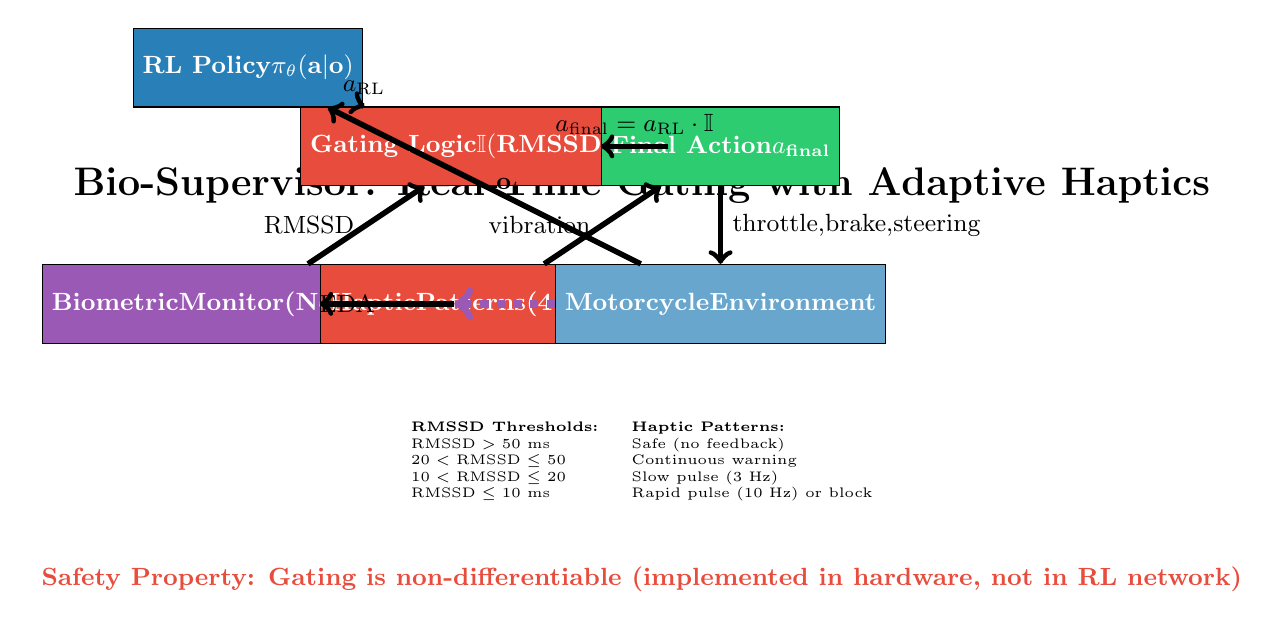
\begin{tikzpicture}[
    node distance=2cm,
]

% Title
\node[draw=none,font=\Large\bfseries] at (7,-0.5) {Bio-Supervisor: Real-Time Gating with Adaptive Haptics};

% RL Policy
\node[draw,fill=pomdpblue,text=white,font=\small\bfseries,minimum width=2.5cm,minimum height=1cm] (rl) at (2,1) {RL Policy\\$\pi_\theta(\mathbf{a}|\mathbf{o})$};

% Biometric Monitor
\node[draw,fill=biomarkerviolet,text=white,font=\small\bfseries,minimum width=2.5cm,minimum height=1cm] (bio) at (2,-2) {Biometric\\Monitor\\(NeuroKit2)};

% Gating logic
\node[draw,fill=hapticsred,text=white,font=\small\bfseries,minimum width=2.5cm,minimum height=1cm] (gating) at (5,0) {Gating Logic\\$\mathbb{I}(\text{RMSSD} > \theta)$};

% Haptic feedback
\node[draw,fill=hapticsred,text=white,font=\small\bfseries,minimum width=2.5cm,minimum height=1cm] (haptic) at (5,-2) {Haptic\\Patterns\\(4-stage)};

% Final action
\node[draw,fill=rewardgreen,text=white,font=\small\bfseries,minimum width=2.5cm,minimum height=1cm] (action) at (8,0) {Final Action\\$a_{\text{final}}$};

% Motorcycle environment
\node[draw,fill=pomdpblue!70,text=white,font=\small\bfseries,minimum width=2.5cm,minimum height=1cm] (env) at (8,-2) {Motorcycle\\Environment};

% Connections
\draw[->,line width=2pt] (rl) -- node[above,draw=none,font=\small] {$a_{\text{RL}}$} (gating);
\draw[->,line width=2pt] (gating) -- node[above,draw=none,font=\small] {$a_{\text{final}} = a_{\text{RL}} \cdot \mathbb{I}$} (action);

\draw[->,line width=2pt] (bio) -- node[left,draw=none,font=\small] {RMSSD} (gating);
\draw[->,line width=2pt] (bio) -- node[left,draw=none,font=\small] {EDA} (haptic);
\draw[->,line width=2pt] (haptic) -- node[left,draw=none,font=\small] {vibration} (action);

\draw[->,line width=2pt] (action) -- node[right,draw=none,font=\small] {throttle,\\brake,\\steering} (env);
\draw[->,line width=3pt,dashed,biomarkerviolet] (env) -- (bio);
\draw[->,line width=2pt] (env) -- node[right,draw=none,font=\small] {$\mathbf{o}_t$} (rl);

% Legend box
\node[draw=none,font=\tiny,inner sep=5pt] at (7,-4) {
\begin{tabular}{ll}
\textbf{RMSSD Thresholds:} & \textbf{Haptic Patterns:} \\
$\text{RMSSD} > 50$ ms & Safe (no feedback) \\
$20 < \text{RMSSD} \leq 50$ & Continuous warning \\
$10 < \text{RMSSD} \leq 20$ & Slow pulse (3 Hz) \\
$\text{RMSSD} \leq 10$ ms & Rapid pulse (10 Hz) or block \\
\end{tabular}
};

\node[draw=none,font=\small\bfseries,text=hapticsred,inner sep=5pt] at (7,-5.5) {\textbf{Safety Property:} Gating is non-differentiable (implemented in hardware, not in RL network)};

\end{tikzpicture}

\pagebreak

% ============================================================================
% FIGURE 4: POLICY ARCHITECTURE WITH BIOMETRIC FUSION
% ============================================================================

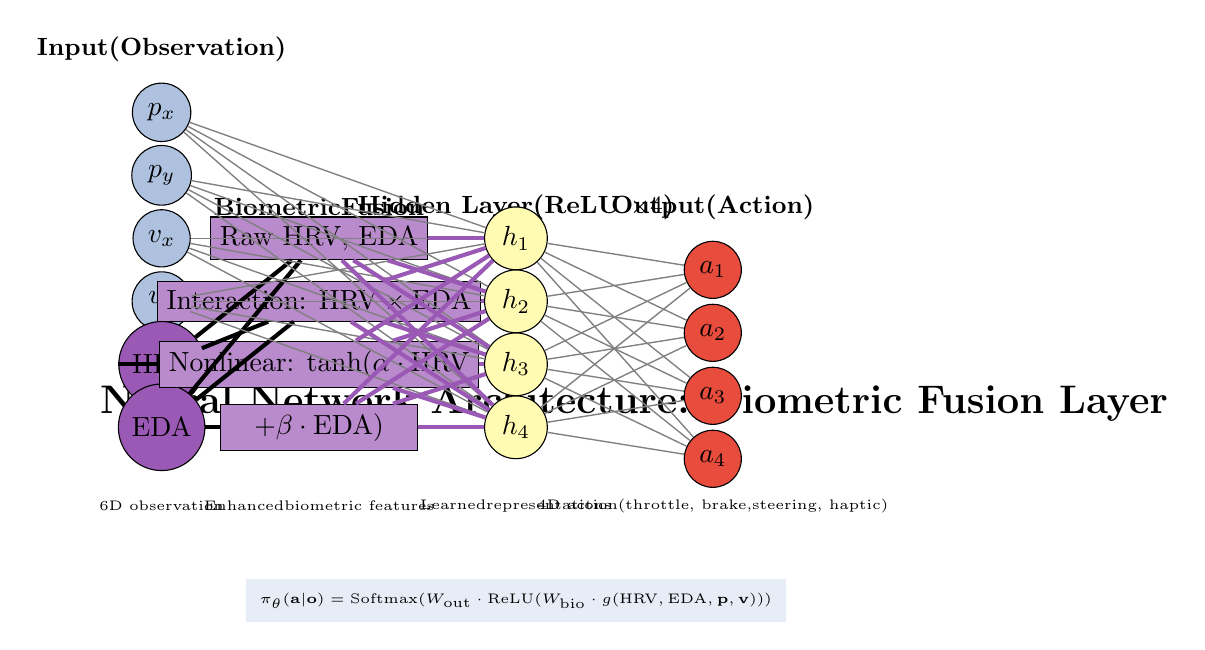
\begin{tikzpicture}[
    node distance=1.5cm,
]

% Title
\node[draw=none,font=\Large\bfseries] at (7,-0.5) {Neural Network Architecture: Biometric Fusion Layer};

% Input layer
\node[draw=none,font=\small\bfseries] at (1,4) {Input\\(Observation)};

\node[draw,fill=lightblue,circle,minimum size=0.6cm] (p1) at (1,3.2) {$p_x$};
\node[draw,fill=lightblue,circle,minimum size=0.6cm] (p2) at (1,2.4) {$p_y$};
\node[draw,fill=lightblue,circle,minimum size=0.6cm] (v1) at (1,1.6) {$v_x$};
\node[draw,fill=lightblue,circle,minimum size=0.6cm] (v2) at (1,0.8) {$v_y$};
\node[draw,fill=biomarkerviolet,circle,minimum size=0.6cm] (hrv) at (1,0) {HRV};
\node[draw,fill=biomarkerviolet,circle,minimum size=0.6cm] (eda) at (1,-0.8) {EDA};

% Biometric fusion layer
\node[draw=none,font=\small\bfseries] at (3,2) {Biometric\\Fusion};

\node[draw,fill=biomarkerviolet!70,rectangle,minimum width=2.5cm,minimum height=0.5cm] (fusion1) at (3,1.6) {Raw HRV, EDA};
\node[draw,fill=biomarkerviolet!70,rectangle,minimum width=2.5cm,minimum height=0.5cm] (fusion2) at (3,0.8) {Interaction: $\text{HRV} \times \text{EDA}$};
\node[draw,fill=biomarkerviolet!70,rectangle,minimum width=2.5cm,minimum height=0.5cm] (fusion3) at (3,0) {Nonlinear: $\tanh(\alpha\cdot\text{HRV}$};
\node[draw,fill=biomarkerviolet!70,rectangle,minimum width=2.5cm,minimum height=0.5cm] (fusion4) at (3,-0.8) {$+\beta\cdot\text{EDA})$};

% Hidden layer
\node[draw=none,font=\small\bfseries] at (5.5,2) {Hidden Layer\\(ReLU $\times 4$)};

\node[draw,fill=yellow!30,circle,minimum size=0.6cm] (h1) at (5.5,1.6) {$h_1$};
\node[draw,fill=yellow!30,circle,minimum size=0.6cm] (h2) at (5.5,0.8) {$h_2$};
\node[draw,fill=yellow!30,circle,minimum size=0.6cm] (h3) at (5.5,0) {$h_3$};
\node[draw,fill=yellow!30,circle,minimum size=0.6cm] (h4) at (5.5,-0.8) {$h_4$};

% Output layer
\node[draw=none,font=\small\bfseries] at (8,2) {Output\\(Action)};

\node[draw,fill=hapticsred,circle,minimum size=0.6cm] (a1) at (8,1.2) {$a_1$};
\node[draw,fill=hapticsred,circle,minimum size=0.6cm] (a2) at (8,0.4) {$a_2$};
\node[draw,fill=hapticsred,circle,minimum size=0.6cm] (a3) at (8,-0.4) {$a_3$};
\node[draw,fill=hapticsred,circle,minimum size=0.6cm] (a4) at (8,-1.2) {$a_4$};

% Connections from input to fusion
\draw[-,line width=1.5pt] (hrv) -- (fusion1);
\draw[-,line width=1.5pt] (eda) -- (fusion1);
\draw[-,line width=1.5pt] (hrv) -- (fusion2);
\draw[-,line width=1.5pt] (eda) -- (fusion2);
\draw[-,line width=1.5pt] (hrv) -- (fusion3);
\draw[-,line width=1.5pt] (eda) -- (fusion4);

% Connections from position/velocity to hidden
\foreach \s in {p1,p2,v1,v2}
    \foreach \h in {h1,h2,h3,h4}
        \draw[-,line width=0.5pt,gray] (\s) -- (\h);

% Connections from fusion to hidden
\foreach \f in {fusion1,fusion2,fusion3,fusion4}
    \foreach \h in {h1,h2,h3,h4}
        \draw[-,line width=1.5pt,biomarkerviolet] (\f) -- (\h);

% Connections from hidden to output
\foreach \h in {h1,h2,h3,h4}
    \foreach \a in {a1,a2,a3,a4}
        \draw[-,line width=0.5pt,gray] (\h) -- (\a);

% Labels
\node[draw=none,font=\tiny] at (1,-1.8) {6D observation};
\node[draw=none,font=\tiny] at (3,-1.8) {Enhanced\\biometric features};
\node[draw=none,font=\tiny] at (5.5,-1.8) {Learned\\representations};
\node[draw=none,font=\tiny] at (8,-1.8) {4D action\\(throttle, brake,\\steering, haptic)};

% Formula box
\node[draw=none,font=\tiny,inner sep=5pt,fill=lightblue!30] at (5.5,-3) {
$\pi_\theta(\mathbf{a}|\mathbf{o}) = \text{Softmax}(W_{\text{out}} \cdot \text{ReLU}(W_{\text{bio}} \cdot g(\text{HRV}, \text{EDA}, \mathbf{p}, \mathbf{v})))$
};

\end{tikzpicture}

\pagebreak

% ============================================================================
% FIGURE 5: RMSSD-BASED COGNITIVE LOAD REWARD
% ============================================================================

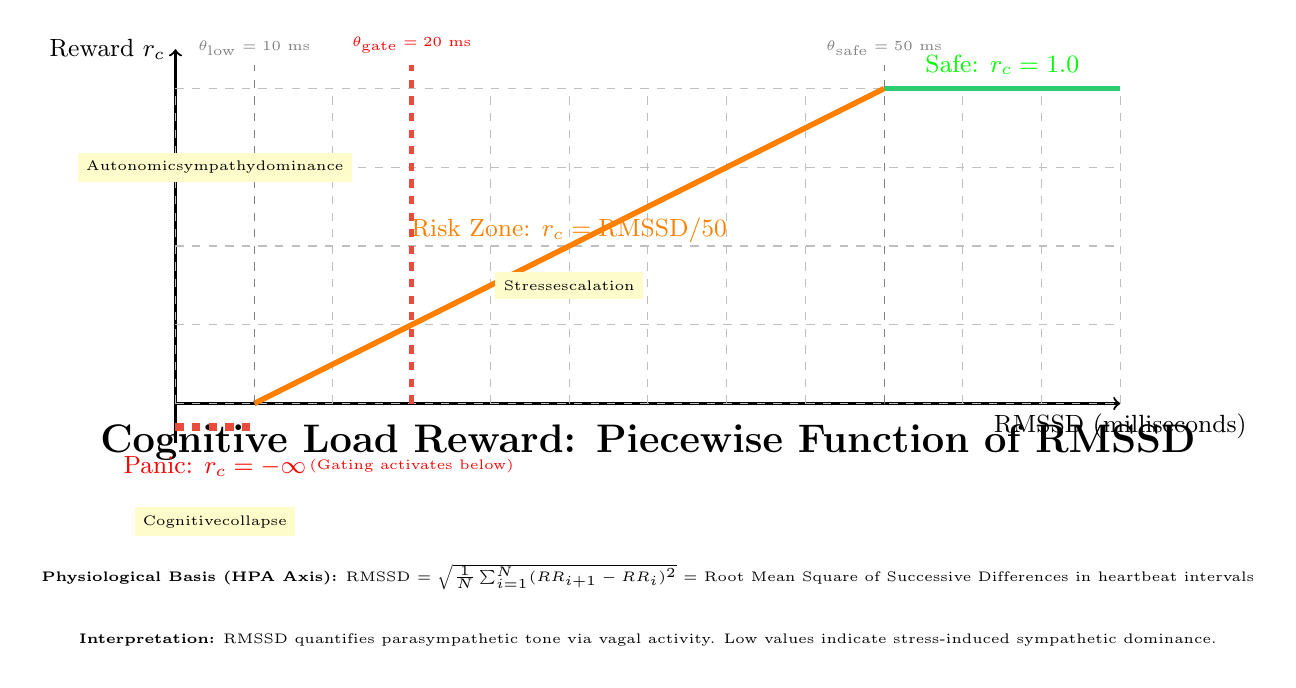
\begin{tikzpicture}

% Title
\node[draw=none,font=\Large\bfseries] at (7,-0.5) {Cognitive Load Reward: Piecewise Function of RMSSD};

% Axes
\draw[thick,->] (1,0) -- (13,0) node[below,font=\small] {RMSSD (milliseconds)};
\draw[thick,->] (1,-0.5) -- (1,4.5) node[left,font=\small] {Reward $r_c$};

% Grid
\draw[dashed,gray!50] (1,0) grid[step=1] (13,4);

% Function pieces
% Safe zone (RMSSD >= 50)
\draw[thick, rewardgreen, line width=2pt] (10,4) -- (13,4);
\node[draw=none,font=\small,text=green] at (11.5,4.3) {Safe: $r_c = 1.0$};

% Linear zone (10 < RMSSD < 50)
\draw[thick, orange, line width=2pt] (2,0) -- (10,4);
\node[draw=none,font=\small,text=orange] at (6,2.2) {Risk Zone: $r_c = \text{RMSSD}/50$};

% Panic zone (RMSSD <= 10)
\draw[thick, hapticsred, line width=3pt, dashed] (1,-0.3) -- (2,-0.3);
\node[draw=none,font=\small,text=red] at (1.5,-0.8) {Panic: $r_c = -\infty$};

% Threshold lines
\draw[dashed, gray] (2,0) -- (2,4.3) node[above,font=\tiny] {$\theta_{\text{low}} = 10$ ms};
\draw[dashed, gray] (10,0) -- (10,4.3) node[above,font=\tiny] {$\theta_{\text{safe}} = 50$ ms};

% Gating threshold
\draw[dashed, hapticsred, line width=2pt] (4,0) -- (4,4.3) node[above,font=\tiny,text=red] {$\theta_{\text{gate}} = 20$ ms};
\node[draw=none,font=\tiny,text=red] at (4,-0.8) {(Gating activates below)};

% Annotations
\node[draw=none,font=\tiny,inner sep=3pt,fill=yellow!20] at (1.5,3) {Autonomic\\sympathy\\dominance};
\node[draw=none,font=\tiny,inner sep=3pt,fill=yellow!20] at (6,1.5) {Stress\\escalation};
\node[draw=none,font=\tiny,inner sep=3pt,fill=yellow!20] at (1.5,-1.5) {Cognitive\\collapse};

% Legend
\node[draw=none,font=\tiny,inner sep=5pt] at (7,-2.2) {
\textbf{Physiological Basis (HPA Axis):}
RMSSD = $\sqrt{\frac{1}{N}\sum_{i=1}^N (RR_{i+1} - RR_i)^2}$ = Root Mean Square of Successive Differences in heartbeat intervals
};

\node[draw=none,font=\tiny,inner sep=5pt] at (7,-3) {
\textbf{Interpretation:} RMSSD quantifies parasympathetic tone via vagal activity. Low values indicate stress-induced sympathetic dominance.
};

\end{tikzpicture}

\pagebreak

% ============================================================================
% FIGURE 6: STATE SPACE DIMENSIONALITY
% ============================================================================

\begin{tikzpicture}

% Title
\node[draw=none,font=\Large\bfseries] at (7,-0.5) {State Space: 7D Hidden vs 6D Observed};

% Hidden state box
\node[draw,fill=pomdpblue,text=white,font=\small\bfseries,minimum width=4cm,minimum height=3cm] (hidden) at (2.5,1.5) {
\begin{tabular}{c}
\textbf{Hidden State} $\mathbf{s}_t \in \mathbb{R}^7$ \\
\\
$p_x$ (position X) \\
$p_y$ (position Y) \\
$v_x$ (velocity X) \\
$v_y$ (velocity Y) \\
HRV (Heart Rate Var.) \\
EDA (Electro. Dermal) \\
$\phi$ (lean angle) \textcolor{red}{???}
\end{tabular}
};

% Observation box
\node[draw,fill=biomarkerviolet,text=white,font=\small\bfseries,minimum width=4cm,minimum height=2.5cm] (obs) at (7.5,1.5) {
\begin{tabular}{c}
\textbf{Observed} $\mathbf{o}_t \in \mathbb{R}^6$ \\
\\
$p_x$ (position X) \\
$p_y$ (position Y) \\
$v_x$ (velocity X) \\
$v_y$ (velocity Y) \\
HRV (Heart Rate Var.) \\
EDA (Electro. Dermal)
\end{tabular}
};

% Arrow showing loss of information
\draw[->,line width=3pt,red] (4.8,2) -- (5.7,2) node[above,draw=none,font=\small,text=red] {Partial\\Observability};

% Explanation
\node[draw=none,font=\small,text=darkred,inner sep=5pt,fill=red!10] at (5,0.3) {
Motorcycle lean angle $\phi$ is \textbf{hidden} from agent \\
(proprioceptive sensing not available in coaching context)
};

% Agent belief
\node[draw,fill=rewardgreen!70,text=white,font=\small\bfseries,minimum width=3cm,minimum height=1.5cm] (belief) at (5,-2.5) {
\begin{tabular}{c}
\textbf{Agent Belief} \\
State via Bayesian Filter \\
$b_t(s_t) = \frac{\mathcal{O}(o_t|s_t) P(s_t|s_{t-1},a_{t-1}) b_{t-1}(s_{t-1})}{\mathcal{O}(o_t)}$
\end{tabular}
};

\draw[->,line width=2pt] (2.5,0.2) -- (belief);
\draw[->,line width=2pt] (7.5,0.2) -- (belief);

\end{tikzpicture}

\pagebreak

% ============================================================================
% FIGURE 7: TRAINING ALGORITHM FLOWCHART
% ============================================================================

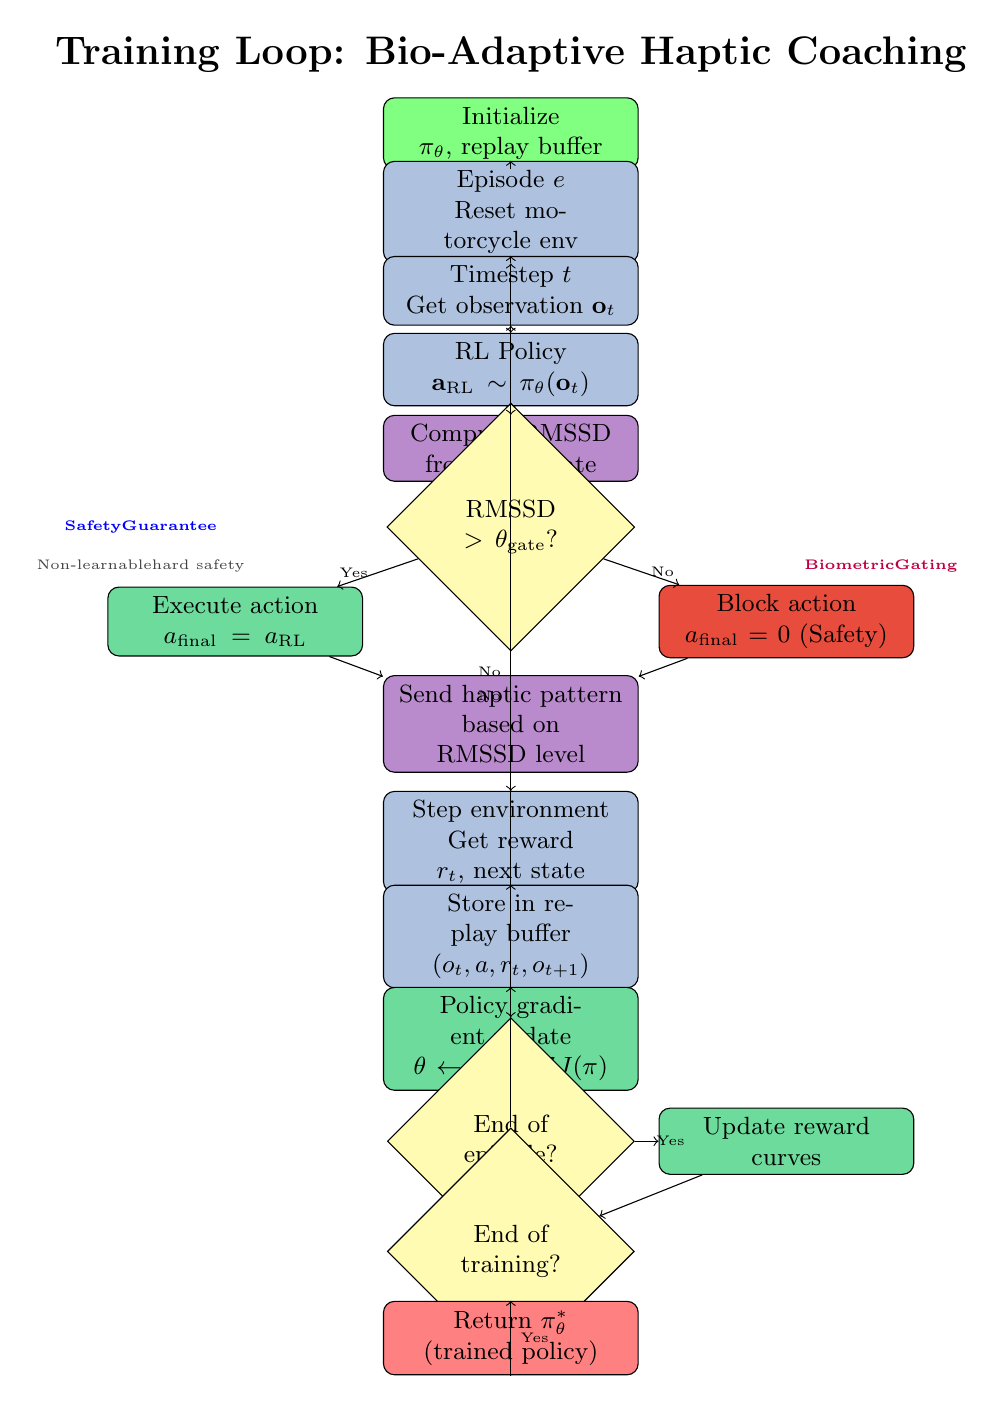
\begin{tikzpicture}[
    node distance=1.8cm,
    block/.style={draw, fill=lightblue, text width=3cm, text centered, rounded corners, minimum height=0.8cm, font=\small},
    decision/.style={diamond, draw, fill=yellow!30, text width=2cm, text centered, minimum height=1cm, font=\small},
    action/.style={draw, fill=rewardgreen!70, text width=3cm, text centered, rounded corners, minimum height=0.8cm, font=\small},
    bioaction/.style={draw, fill=biomarkerviolet!70, text width=3cm, text centered, rounded corners, minimum height=0.8cm, font=\small}
]

% Title
\node[draw=none,font=\Large\bfseries] at (5,9) {Training Loop: Bio-Adaptive Haptic Coaching};

% Start
\node[block,fill=green!50] (start) at (5,8) {Initialize\\$\pi_\theta$, replay buffer};

% Episode
\node[block] (episode) at (5,7) {Episode $e$\\Reset motorcycle env};

% Timestep
\node[block] (timestep) at (5,6) {Timestep $t$\\Get observation $\mathbf{o}_t$};

% Action selection
\node[block] (action) at (5,5) {RL Policy\\$\mathbf{a}_{\text{RL}} \sim \pi_\theta(\mathbf{o}_t)$};

% Compute RMSSD
\node[bioaction] (rmssd) at (5,4) {Compute RMSSD\\from heart rate};

% Gating decision
\node[decision] (gate) at (5,3) {RMSSD\\$> \theta_{\text{gate}}$?};

% Gating true
\node[action] (gate_true) at (1.5,1.8) {Execute action\\$a_{\text{final}} = a_{\text{RL}}$};

% Gating false
\node[action,fill=hapticsred] (gate_false) at (8.5,1.8) {Block action\\$a_{\text{final}} = 0$ (Safety)};

% Haptic feedback
\node[bioaction] (haptic) at (5,0.5) {Send haptic pattern\\based on RMSSD level};

% Step environment
\node[block] (step) at (5,-1) {Step environment\\Get reward $r_t$, next state};

% Store transition
\node[block] (store) at (5,-2.2) {Store in replay buffer\\$(o_t, a, r_t, o_{t+1})$};

% Update policy
\node[action] (update) at (5,-3.5) {Policy gradient update\\$\theta \leftarrow \theta + \alpha \nabla J(\pi)$};

% End of episode?
\node[decision] (eod) at (5,-4.8) {End of\\episode?};

% Update curves
\node[action] (curves) at (8.5,-4.8) {Update reward\\curves};

% End training?
\node[decision] (eot) at (5,-6.2) {End of\\training?};

% End
\node[block,fill=red!50] (end) at (5,-7.3) {Return $\pi_\theta^*$\\(trained policy)};

% Connections
\draw[->] (start) -- (episode);
\draw[->] (episode) -- (timestep);
\draw[->] (timestep) -- (action);
\draw[->] (action) -- (rmssd);
\draw[->] (rmssd) -- (gate);

\draw[->] (gate) -- node[left,draw=none,font=\tiny] {Yes} (gate_true);
\draw[->] (gate) -- node[right,draw=none,font=\tiny] {No} (gate_false);

\draw[->] (gate_true) -- (haptic);
\draw[->] (gate_false) -- (haptic);

\draw[->] (haptic) -- (step);
\draw[->] (step) -- (store);
\draw[->] (store) -- (update);

\draw[->] (update) -- (eod);
\draw[->] (eod) -- node[left,draw=none,font=\tiny] {No} (timestep);
\draw[->] (eod) -- node[right,draw=none,font=\tiny] {Yes} (curves);

\draw[->] (curves) -- (eot);
\draw[->] (eot) -- node[left,draw=none,font=\tiny] {No} (episode);
\draw[->] (eot) -- node[right,draw=none,font=\tiny] {Yes} (end);

% Side notes
\node[draw=none,font=\tiny,text=blue,inner sep=3pt] at (0.3,3) {\textbf{Safety\\Guarantee}};
\node[draw=none,font=\tiny,text=darkgray] at (0.3,2.5) {Non-learnable\\hard safety};

\node[draw=none,font=\tiny,text=purple,inner sep=3pt] at (9.7,2.5) {\textbf{Biometric\\Gating}};

\end{tikzpicture}

\end{document}
 in your main document

\documentclass[12pt,border=5pt]{standalone}
\usepackage{tikz}
\usepackage{amsmath}
\usepackage{amssymb}

\usetikzlibrary{shapes,arrows,positioning,calc,fit,decorations.pathmorphing}

% Color scheme
\definecolor{pomdpblue}{RGB}{41,128,185}
\definecolor{rewardgreen}{RGB}{46,204,113}
\definecolor{hapticsred}{RGB}{231,76,60}
\definecolor{biomarkerviolet}{RGB}{155,89,182}
\definecolor{lightblue}{RGB}{174,194,224}
\definecolor{lightgreen}{RGB}{154,235,206}

% ============================================================================
% FIGURE 1: POMDP STRUCTURE WITH BIOMETRIC STATE
% ============================================================================

\begin{document}

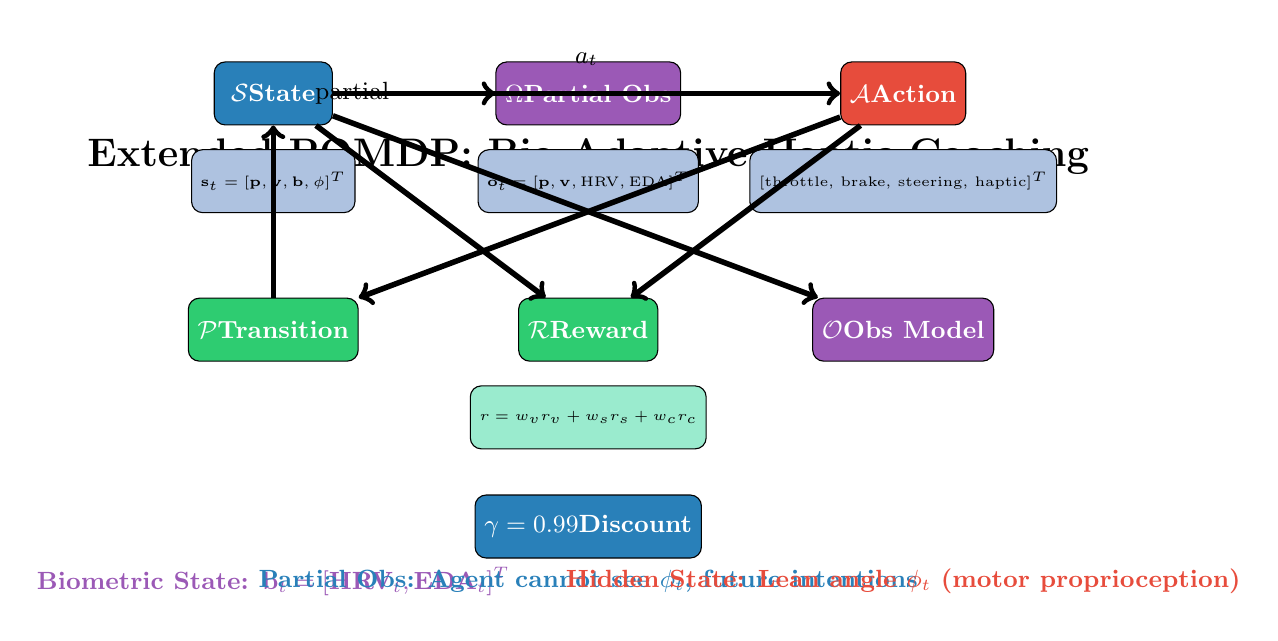
\begin{tikzpicture}[
    node distance=2.5cm,
    every node/.style={draw,rounded corners,minimum width=1.5cm,minimum height=0.8cm,font=\small\bfseries}
]

% Title
\node[draw=none,font=\Large\bfseries] at (6,-0.8) {Extended POMDP: Bio-Adaptive Haptic Coaching};

% State space
\node[fill=pomdpblue,text=white] (state) at (2,0) {$\mathcal{S}$\\State};
\node[fill=lightblue,text=black,below=0.3cm of state,draw,font=\tiny,rounded corners] {$\mathbf{s}_t = [\mathbf{p}, \mathbf{v}, \mathbf{b}, \phi]^T$};

% Observation space (partial)
\node[fill=biomarkerviolet,text=white] (obs) at (6,0) {$\Omega$\\Partial Obs};
\node[fill=lightblue,text=black,below=0.3cm of obs,draw,font=\tiny,rounded corners] {$\mathbf{o}_t = [\mathbf{p}, \mathbf{v}, \text{HRV}, \text{EDA}]^T$};

% Action space
\node[fill=hapticsred,text=white] (action) at (10,0) {$\mathcal{A}$\\Action};
\node[fill=lightblue,text=black,below=0.3cm of action,draw,font=\tiny,rounded corners] {$[\text{throttle, brake, steering, haptic}]^T$};

% Transition model
\node[fill=rewardgreen,text=white] (trans) at (2,-3) {$\mathcal{P}$\\Transition};

% Reward function
\node[fill=rewardgreen,text=white] (reward) at (6,-3) {$\mathcal{R}$\\Reward};
\node[fill=lightgreen,text=black,below=0.3cm of reward,draw,font=\tiny,rounded corners] {$r = w_v r_v + w_s r_s + w_c r_c$};

% Observation model
\node[fill=biomarkerviolet,text=white] (obsmodel) at (10,-3) {$\mathcal{O}$\\Obs Model};

% Discount factor
\node[fill=pomdpblue,text=white] (discount) at (6,-5.5) {$\gamma = 0.99$\\Discount};

% Connections
\draw[->,line width=2pt] (state) -- node[above,draw=none,font=\small] {$a_t$} (action);
\draw[->,line width=2pt] (action) -- (trans);
\draw[->,line width=2pt] (trans) -- (state);
\draw[->,line width=2pt] (state) -- (reward);
\draw[->,line width=2pt] (action) -- (reward);
\draw[->,line width=2pt] (state) -- node[left,draw=none,font=\small] {partial} (obs);
\draw[->,line width=2pt] (state) -- (obsmodel);

% Biometric component highlight
\node[draw=none,font=\small\bfseries,text=biomarkerviolet] at (2,-6.2) {\textbf{Biometric State:} $\mathbf{b}_t = [\text{HRV}_t, \text{EDA}_t]^T$};
\node[draw=none,font=\small\bfseries,text=pomdpblue] at (6,-6.2) {\textbf{Partial Obs:} Agent cannot see $\phi_t$, future intentions};
\node[draw=none,font=\small\bfseries,text=hapticsred] at (10,-6.2) {\textbf{Hidden State:} Lean angle $\phi_t$ (motor proprioception)};

\end{tikzpicture}

\pagebreak

% ============================================================================
% FIGURE 2: MULTI-OBJECTIVE REWARD SCALARIZATION
% ============================================================================

\begin{tikzpicture}

% Title
\node[draw=none,font=\Large\bfseries] at (7,-0.5) {Multi-Objective Reward Scalarization};

% Velocity reward
\begin{scope}[shift=(0,0)]
\node[fill=rewardgreen,text=white,font=\small\bfseries] at (2,2) {$r_v$ (Velocity)};
\draw[thick, rewardgreen] (0.5,0) -- (1,0.3) -- (2,0.8) -- (3,1.2) -- (3.5,1.5);
\draw[dashed,gray] (0,0) -- (4,0) -- (4,2) -- (0,2) -- (0,0);
\node[draw=none,font=\tiny] at (2,-0.4) {Speed $\rightarrow$};
\node[draw=none,font=\tiny] at (-0.5,1) {Reward};
\node[draw=none,font=\tiny] at (2,-0.8) {Weight: $w_v = 0.50$};
\end{scope}

% Safety reward
\begin{scope}[shift=(5,0)]
\node[fill=rewardgreen,text=white,font=\small\bfseries] at (2,2) {$r_s$ (Safety)};
\draw[thick, rewardgreen] (0.5,0.05) -- (1,0.3) -- (2,0.8) -- (3,1.3) -- (3.5,1.45);
\draw[dashed,gray] (0,0) -- (4,0) -- (4,2) -- (0,2) -- (0,0);
\node[draw=none,font=\tiny] at (2,-0.4) {Distance to obstacle};
\node[draw=none,font=\tiny] at (-0.5,1) {Reward};
\node[draw=none,font=\tiny] at (2,-0.8) {Weight: $w_s = 0.35$};
\end{scope}

% Cognitive Load reward
\begin{scope}[shift=(10,0)]
\node[fill=biomarkerviolet,text=white,font=\small\bfseries] at (2,2) {$r_c$ (Cog Load)};
% Safe zone
\draw[thick, biomarkerviolet] (0.5,1.5) -- (1.8,1.5);
% Risk zone
\draw[thick, biomarkerviolet] (1.8,1.5) -- (3,0.3);
% Panic zone
\draw[thick, biomarkerviolet, dashed] (3,0.3) -- (3.5,-0.5);
\draw[dashed,gray] (0,0) -- (4,0) -- (4,2) -- (0,2) -- (0,0);
\node[draw=none,font=\tiny,text=green] at (1.2,1.8) {RMSSD>50};
\node[draw=none,font=\tiny,text=orange] at (2.5,0.8) {10-50};
\node[draw=none,font=\tiny,text=red] at (3.2,-0.2) {<10};
\node[draw=none,font=\tiny] at (-0.5,1) {Reward};
\node[draw=none,font=\tiny] at (2,-0.8) {Weight: $w_c = 0.15$};
\end{scope}

% Weighted combination
\node[draw=none,font=\normalsize\bfseries,fill=yellow!20,inner sep=10pt] at (7,-2.5) {$r_t = 0.50 \cdot r_v + 0.35 \cdot r_s + 0.15 \cdot r_c$};

\node[draw=none,font=\tiny,text=darkgray,inner sep=5pt] at (7,-3.3) {Objective function: $J(\pi) = \mathbb{E}[\sum_t \gamma^t r_t]$ maximized by policy gradient};

\end{tikzpicture}

\pagebreak

% ============================================================================
% FIGURE 3: BIO-SUPERVISOR ARCHITECTURE
% ============================================================================

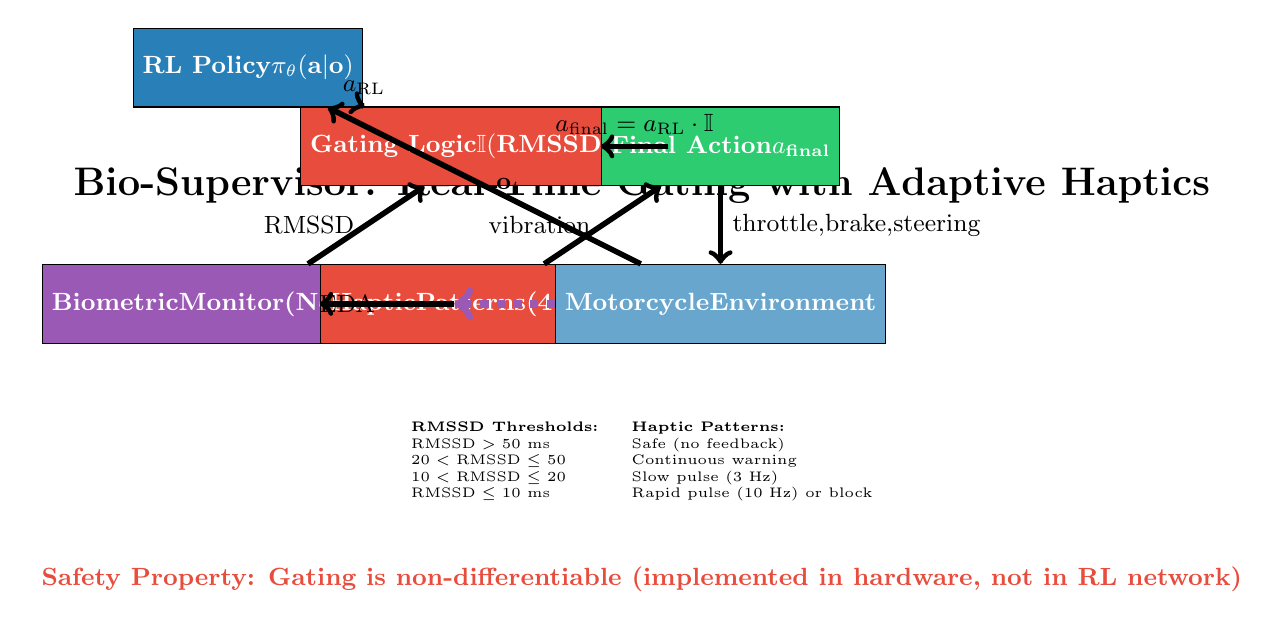
\begin{tikzpicture}[
    node distance=2cm,
]

% Title
\node[draw=none,font=\Large\bfseries] at (7,-0.5) {Bio-Supervisor: Real-Time Gating with Adaptive Haptics};

% RL Policy
\node[draw,fill=pomdpblue,text=white,font=\small\bfseries,minimum width=2.5cm,minimum height=1cm] (rl) at (2,1) {RL Policy\\$\pi_\theta(\mathbf{a}|\mathbf{o})$};

% Biometric Monitor
\node[draw,fill=biomarkerviolet,text=white,font=\small\bfseries,minimum width=2.5cm,minimum height=1cm] (bio) at (2,-2) {Biometric\\Monitor\\(NeuroKit2)};

% Gating logic
\node[draw,fill=hapticsred,text=white,font=\small\bfseries,minimum width=2.5cm,minimum height=1cm] (gating) at (5,0) {Gating Logic\\$\mathbb{I}(\text{RMSSD} > \theta)$};

% Haptic feedback
\node[draw,fill=hapticsred,text=white,font=\small\bfseries,minimum width=2.5cm,minimum height=1cm] (haptic) at (5,-2) {Haptic\\Patterns\\(4-stage)};

% Final action
\node[draw,fill=rewardgreen,text=white,font=\small\bfseries,minimum width=2.5cm,minimum height=1cm] (action) at (8,0) {Final Action\\$a_{\text{final}}$};

% Motorcycle environment
\node[draw,fill=pomdpblue!70,text=white,font=\small\bfseries,minimum width=2.5cm,minimum height=1cm] (env) at (8,-2) {Motorcycle\\Environment};

% Connections
\draw[->,line width=2pt] (rl) -- node[above,draw=none,font=\small] {$a_{\text{RL}}$} (gating);
\draw[->,line width=2pt] (gating) -- node[above,draw=none,font=\small] {$a_{\text{final}} = a_{\text{RL}} \cdot \mathbb{I}$} (action);

\draw[->,line width=2pt] (bio) -- node[left,draw=none,font=\small] {RMSSD} (gating);
\draw[->,line width=2pt] (bio) -- node[left,draw=none,font=\small] {EDA} (haptic);
\draw[->,line width=2pt] (haptic) -- node[left,draw=none,font=\small] {vibration} (action);

\draw[->,line width=2pt] (action) -- node[right,draw=none,font=\small] {throttle,\\brake,\\steering} (env);
\draw[->,line width=3pt,dashed,biomarkerviolet] (env) -- (bio);
\draw[->,line width=2pt] (env) -- node[right,draw=none,font=\small] {$\mathbf{o}_t$} (rl);

% Legend box
\node[draw=none,font=\tiny,inner sep=5pt] at (7,-4) {
\begin{tabular}{ll}
\textbf{RMSSD Thresholds:} & \textbf{Haptic Patterns:} \\
$\text{RMSSD} > 50$ ms & Safe (no feedback) \\
$20 < \text{RMSSD} \leq 50$ & Continuous warning \\
$10 < \text{RMSSD} \leq 20$ & Slow pulse (3 Hz) \\
$\text{RMSSD} \leq 10$ ms & Rapid pulse (10 Hz) or block \\
\end{tabular}
};

\node[draw=none,font=\small\bfseries,text=hapticsred,inner sep=5pt] at (7,-5.5) {\textbf{Safety Property:} Gating is non-differentiable (implemented in hardware, not in RL network)};

\end{tikzpicture}

\pagebreak

% ============================================================================
% FIGURE 4: POLICY ARCHITECTURE WITH BIOMETRIC FUSION
% ============================================================================

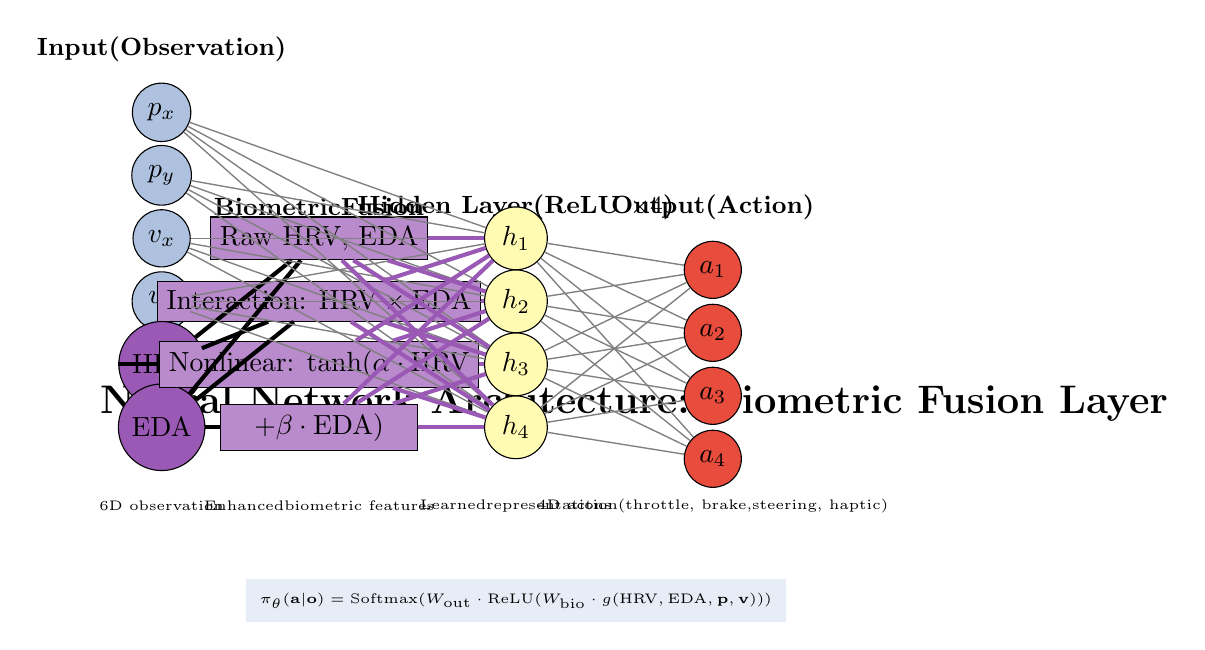
\begin{tikzpicture}[
    node distance=1.5cm,
]

% Title
\node[draw=none,font=\Large\bfseries] at (7,-0.5) {Neural Network Architecture: Biometric Fusion Layer};

% Input layer
\node[draw=none,font=\small\bfseries] at (1,4) {Input\\(Observation)};

\node[draw,fill=lightblue,circle,minimum size=0.6cm] (p1) at (1,3.2) {$p_x$};
\node[draw,fill=lightblue,circle,minimum size=0.6cm] (p2) at (1,2.4) {$p_y$};
\node[draw,fill=lightblue,circle,minimum size=0.6cm] (v1) at (1,1.6) {$v_x$};
\node[draw,fill=lightblue,circle,minimum size=0.6cm] (v2) at (1,0.8) {$v_y$};
\node[draw,fill=biomarkerviolet,circle,minimum size=0.6cm] (hrv) at (1,0) {HRV};
\node[draw,fill=biomarkerviolet,circle,minimum size=0.6cm] (eda) at (1,-0.8) {EDA};

% Biometric fusion layer
\node[draw=none,font=\small\bfseries] at (3,2) {Biometric\\Fusion};

\node[draw,fill=biomarkerviolet!70,rectangle,minimum width=2.5cm,minimum height=0.5cm] (fusion1) at (3,1.6) {Raw HRV, EDA};
\node[draw,fill=biomarkerviolet!70,rectangle,minimum width=2.5cm,minimum height=0.5cm] (fusion2) at (3,0.8) {Interaction: $\text{HRV} \times \text{EDA}$};
\node[draw,fill=biomarkerviolet!70,rectangle,minimum width=2.5cm,minimum height=0.5cm] (fusion3) at (3,0) {Nonlinear: $\tanh(\alpha\cdot\text{HRV}$};
\node[draw,fill=biomarkerviolet!70,rectangle,minimum width=2.5cm,minimum height=0.5cm] (fusion4) at (3,-0.8) {$+\beta\cdot\text{EDA})$};

% Hidden layer
\node[draw=none,font=\small\bfseries] at (5.5,2) {Hidden Layer\\(ReLU $\times 4$)};

\node[draw,fill=yellow!30,circle,minimum size=0.6cm] (h1) at (5.5,1.6) {$h_1$};
\node[draw,fill=yellow!30,circle,minimum size=0.6cm] (h2) at (5.5,0.8) {$h_2$};
\node[draw,fill=yellow!30,circle,minimum size=0.6cm] (h3) at (5.5,0) {$h_3$};
\node[draw,fill=yellow!30,circle,minimum size=0.6cm] (h4) at (5.5,-0.8) {$h_4$};

% Output layer
\node[draw=none,font=\small\bfseries] at (8,2) {Output\\(Action)};

\node[draw,fill=hapticsred,circle,minimum size=0.6cm] (a1) at (8,1.2) {$a_1$};
\node[draw,fill=hapticsred,circle,minimum size=0.6cm] (a2) at (8,0.4) {$a_2$};
\node[draw,fill=hapticsred,circle,minimum size=0.6cm] (a3) at (8,-0.4) {$a_3$};
\node[draw,fill=hapticsred,circle,minimum size=0.6cm] (a4) at (8,-1.2) {$a_4$};

% Connections from input to fusion
\draw[-,line width=1.5pt] (hrv) -- (fusion1);
\draw[-,line width=1.5pt] (eda) -- (fusion1);
\draw[-,line width=1.5pt] (hrv) -- (fusion2);
\draw[-,line width=1.5pt] (eda) -- (fusion2);
\draw[-,line width=1.5pt] (hrv) -- (fusion3);
\draw[-,line width=1.5pt] (eda) -- (fusion4);

% Connections from position/velocity to hidden
\foreach \s in {p1,p2,v1,v2}
    \foreach \h in {h1,h2,h3,h4}
        \draw[-,line width=0.5pt,gray] (\s) -- (\h);

% Connections from fusion to hidden
\foreach \f in {fusion1,fusion2,fusion3,fusion4}
    \foreach \h in {h1,h2,h3,h4}
        \draw[-,line width=1.5pt,biomarkerviolet] (\f) -- (\h);

% Connections from hidden to output
\foreach \h in {h1,h2,h3,h4}
    \foreach \a in {a1,a2,a3,a4}
        \draw[-,line width=0.5pt,gray] (\h) -- (\a);

% Labels
\node[draw=none,font=\tiny] at (1,-1.8) {6D observation};
\node[draw=none,font=\tiny] at (3,-1.8) {Enhanced\\biometric features};
\node[draw=none,font=\tiny] at (5.5,-1.8) {Learned\\representations};
\node[draw=none,font=\tiny] at (8,-1.8) {4D action\\(throttle, brake,\\steering, haptic)};

% Formula box
\node[draw=none,font=\tiny,inner sep=5pt,fill=lightblue!30] at (5.5,-3) {
$\pi_\theta(\mathbf{a}|\mathbf{o}) = \text{Softmax}(W_{\text{out}} \cdot \text{ReLU}(W_{\text{bio}} \cdot g(\text{HRV}, \text{EDA}, \mathbf{p}, \mathbf{v})))$
};

\end{tikzpicture}

\pagebreak

% ============================================================================
% FIGURE 5: RMSSD-BASED COGNITIVE LOAD REWARD
% ============================================================================

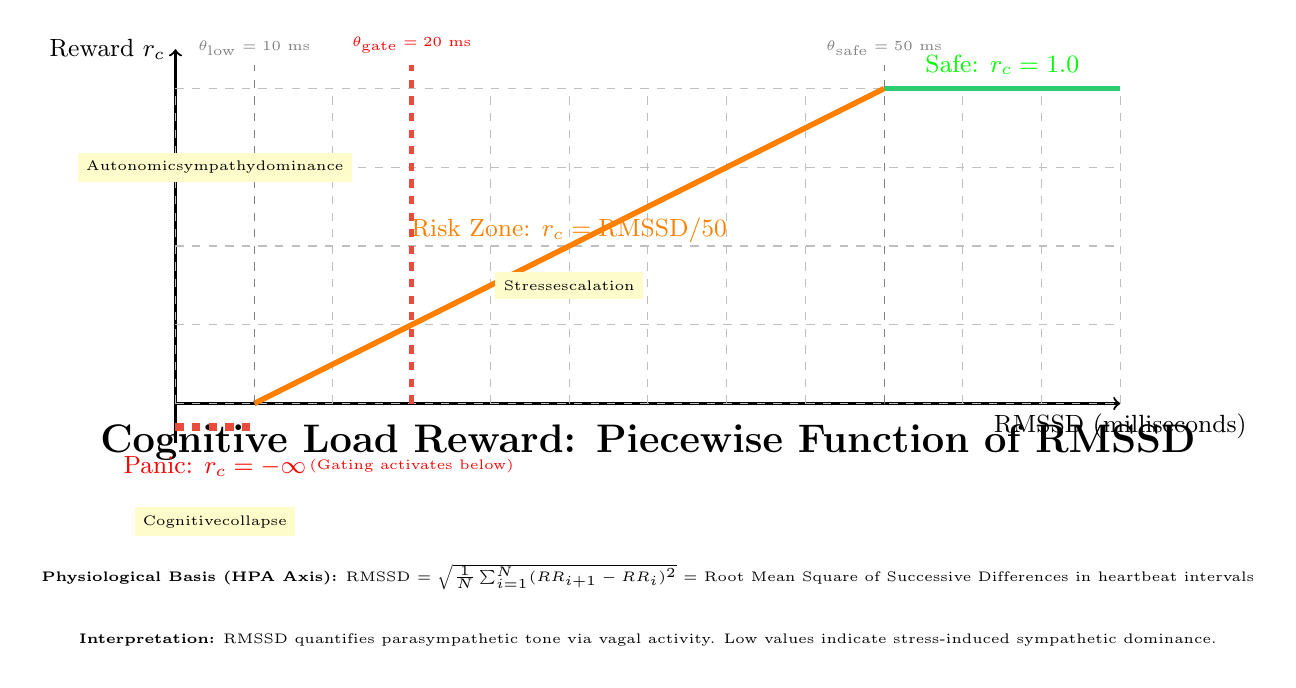
\begin{tikzpicture}

% Title
\node[draw=none,font=\Large\bfseries] at (7,-0.5) {Cognitive Load Reward: Piecewise Function of RMSSD};

% Axes
\draw[thick,->] (1,0) -- (13,0) node[below,font=\small] {RMSSD (milliseconds)};
\draw[thick,->] (1,-0.5) -- (1,4.5) node[left,font=\small] {Reward $r_c$};

% Grid
\draw[dashed,gray!50] (1,0) grid[step=1] (13,4);

% Function pieces
% Safe zone (RMSSD >= 50)
\draw[thick, rewardgreen, line width=2pt] (10,4) -- (13,4);
\node[draw=none,font=\small,text=green] at (11.5,4.3) {Safe: $r_c = 1.0$};

% Linear zone (10 < RMSSD < 50)
\draw[thick, orange, line width=2pt] (2,0) -- (10,4);
\node[draw=none,font=\small,text=orange] at (6,2.2) {Risk Zone: $r_c = \text{RMSSD}/50$};

% Panic zone (RMSSD <= 10)
\draw[thick, hapticsred, line width=3pt, dashed] (1,-0.3) -- (2,-0.3);
\node[draw=none,font=\small,text=red] at (1.5,-0.8) {Panic: $r_c = -\infty$};

% Threshold lines
\draw[dashed, gray] (2,0) -- (2,4.3) node[above,font=\tiny] {$\theta_{\text{low}} = 10$ ms};
\draw[dashed, gray] (10,0) -- (10,4.3) node[above,font=\tiny] {$\theta_{\text{safe}} = 50$ ms};

% Gating threshold
\draw[dashed, hapticsred, line width=2pt] (4,0) -- (4,4.3) node[above,font=\tiny,text=red] {$\theta_{\text{gate}} = 20$ ms};
\node[draw=none,font=\tiny,text=red] at (4,-0.8) {(Gating activates below)};

% Annotations
\node[draw=none,font=\tiny,inner sep=3pt,fill=yellow!20] at (1.5,3) {Autonomic\\sympathy\\dominance};
\node[draw=none,font=\tiny,inner sep=3pt,fill=yellow!20] at (6,1.5) {Stress\\escalation};
\node[draw=none,font=\tiny,inner sep=3pt,fill=yellow!20] at (1.5,-1.5) {Cognitive\\collapse};

% Legend
\node[draw=none,font=\tiny,inner sep=5pt] at (7,-2.2) {
\textbf{Physiological Basis (HPA Axis):}
RMSSD = $\sqrt{\frac{1}{N}\sum_{i=1}^N (RR_{i+1} - RR_i)^2}$ = Root Mean Square of Successive Differences in heartbeat intervals
};

\node[draw=none,font=\tiny,inner sep=5pt] at (7,-3) {
\textbf{Interpretation:} RMSSD quantifies parasympathetic tone via vagal activity. Low values indicate stress-induced sympathetic dominance.
};

\end{tikzpicture}

\pagebreak

% ============================================================================
% FIGURE 6: STATE SPACE DIMENSIONALITY
% ============================================================================

\begin{tikzpicture}

% Title
\node[draw=none,font=\Large\bfseries] at (7,-0.5) {State Space: 7D Hidden vs 6D Observed};

% Hidden state box
\node[draw,fill=pomdpblue,text=white,font=\small\bfseries,minimum width=4cm,minimum height=3cm] (hidden) at (2.5,1.5) {
\begin{tabular}{c}
\textbf{Hidden State} $\mathbf{s}_t \in \mathbb{R}^7$ \\
\\
$p_x$ (position X) \\
$p_y$ (position Y) \\
$v_x$ (velocity X) \\
$v_y$ (velocity Y) \\
HRV (Heart Rate Var.) \\
EDA (Electro. Dermal) \\
$\phi$ (lean angle) \textcolor{red}{???}
\end{tabular}
};

% Observation box
\node[draw,fill=biomarkerviolet,text=white,font=\small\bfseries,minimum width=4cm,minimum height=2.5cm] (obs) at (7.5,1.5) {
\begin{tabular}{c}
\textbf{Observed} $\mathbf{o}_t \in \mathbb{R}^6$ \\
\\
$p_x$ (position X) \\
$p_y$ (position Y) \\
$v_x$ (velocity X) \\
$v_y$ (velocity Y) \\
HRV (Heart Rate Var.) \\
EDA (Electro. Dermal)
\end{tabular}
};

% Arrow showing loss of information
\draw[->,line width=3pt,red] (4.8,2) -- (5.7,2) node[above,draw=none,font=\small,text=red] {Partial\\Observability};

% Explanation
\node[draw=none,font=\small,text=darkred,inner sep=5pt,fill=red!10] at (5,0.3) {
Motorcycle lean angle $\phi$ is \textbf{hidden} from agent \\
(proprioceptive sensing not available in coaching context)
};

% Agent belief
\node[draw,fill=rewardgreen!70,text=white,font=\small\bfseries,minimum width=3cm,minimum height=1.5cm] (belief) at (5,-2.5) {
\begin{tabular}{c}
\textbf{Agent Belief} \\
State via Bayesian Filter \\
$b_t(s_t) = \frac{\mathcal{O}(o_t|s_t) P(s_t|s_{t-1},a_{t-1}) b_{t-1}(s_{t-1})}{\mathcal{O}(o_t)}$
\end{tabular}
};

\draw[->,line width=2pt] (2.5,0.2) -- (belief);
\draw[->,line width=2pt] (7.5,0.2) -- (belief);

\end{tikzpicture}

\pagebreak

% ============================================================================
% FIGURE 7: TRAINING ALGORITHM FLOWCHART
% ============================================================================

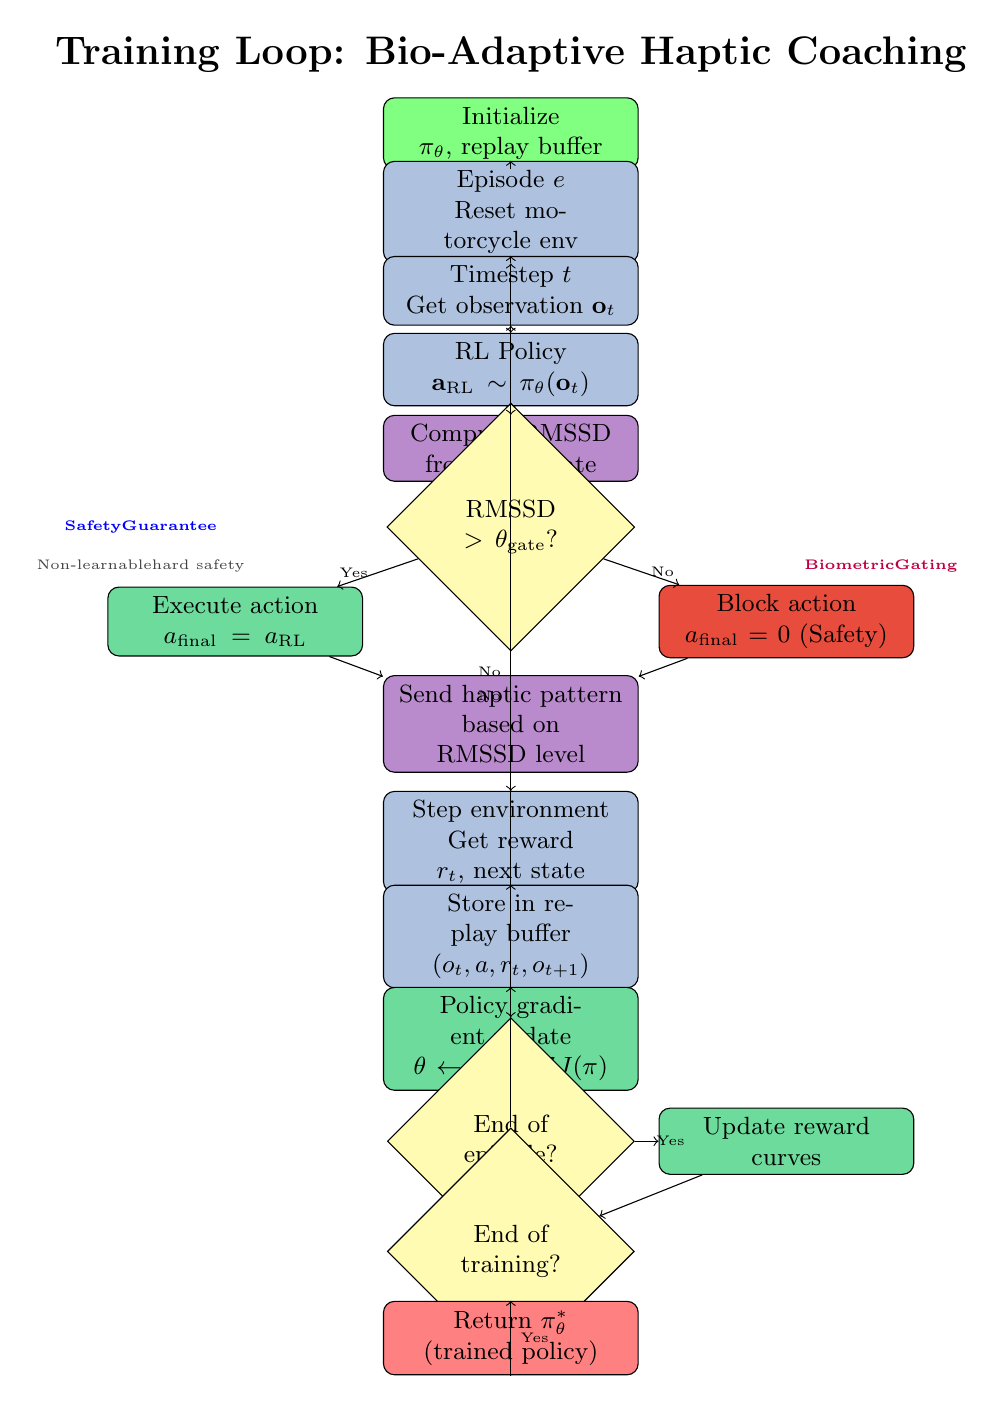
\begin{tikzpicture}[
    node distance=1.8cm,
    block/.style={draw, fill=lightblue, text width=3cm, text centered, rounded corners, minimum height=0.8cm, font=\small},
    decision/.style={diamond, draw, fill=yellow!30, text width=2cm, text centered, minimum height=1cm, font=\small},
    action/.style={draw, fill=rewardgreen!70, text width=3cm, text centered, rounded corners, minimum height=0.8cm, font=\small},
    bioaction/.style={draw, fill=biomarkerviolet!70, text width=3cm, text centered, rounded corners, minimum height=0.8cm, font=\small}
]

% Title
\node[draw=none,font=\Large\bfseries] at (5,9) {Training Loop: Bio-Adaptive Haptic Coaching};

% Start
\node[block,fill=green!50] (start) at (5,8) {Initialize\\$\pi_\theta$, replay buffer};

% Episode
\node[block] (episode) at (5,7) {Episode $e$\\Reset motorcycle env};

% Timestep
\node[block] (timestep) at (5,6) {Timestep $t$\\Get observation $\mathbf{o}_t$};

% Action selection
\node[block] (action) at (5,5) {RL Policy\\$\mathbf{a}_{\text{RL}} \sim \pi_\theta(\mathbf{o}_t)$};

% Compute RMSSD
\node[bioaction] (rmssd) at (5,4) {Compute RMSSD\\from heart rate};

% Gating decision
\node[decision] (gate) at (5,3) {RMSSD\\$> \theta_{\text{gate}}$?};

% Gating true
\node[action] (gate_true) at (1.5,1.8) {Execute action\\$a_{\text{final}} = a_{\text{RL}}$};

% Gating false
\node[action,fill=hapticsred] (gate_false) at (8.5,1.8) {Block action\\$a_{\text{final}} = 0$ (Safety)};

% Haptic feedback
\node[bioaction] (haptic) at (5,0.5) {Send haptic pattern\\based on RMSSD level};

% Step environment
\node[block] (step) at (5,-1) {Step environment\\Get reward $r_t$, next state};

% Store transition
\node[block] (store) at (5,-2.2) {Store in replay buffer\\$(o_t, a, r_t, o_{t+1})$};

% Update policy
\node[action] (update) at (5,-3.5) {Policy gradient update\\$\theta \leftarrow \theta + \alpha \nabla J(\pi)$};

% End of episode?
\node[decision] (eod) at (5,-4.8) {End of\\episode?};

% Update curves
\node[action] (curves) at (8.5,-4.8) {Update reward\\curves};

% End training?
\node[decision] (eot) at (5,-6.2) {End of\\training?};

% End
\node[block,fill=red!50] (end) at (5,-7.3) {Return $\pi_\theta^*$\\(trained policy)};

% Connections
\draw[->] (start) -- (episode);
\draw[->] (episode) -- (timestep);
\draw[->] (timestep) -- (action);
\draw[->] (action) -- (rmssd);
\draw[->] (rmssd) -- (gate);

\draw[->] (gate) -- node[left,draw=none,font=\tiny] {Yes} (gate_true);
\draw[->] (gate) -- node[right,draw=none,font=\tiny] {No} (gate_false);

\draw[->] (gate_true) -- (haptic);
\draw[->] (gate_false) -- (haptic);

\draw[->] (haptic) -- (step);
\draw[->] (step) -- (store);
\draw[->] (store) -- (update);

\draw[->] (update) -- (eod);
\draw[->] (eod) -- node[left,draw=none,font=\tiny] {No} (timestep);
\draw[->] (eod) -- node[right,draw=none,font=\tiny] {Yes} (curves);

\draw[->] (curves) -- (eot);
\draw[->] (eot) -- node[left,draw=none,font=\tiny] {No} (episode);
\draw[->] (eot) -- node[right,draw=none,font=\tiny] {Yes} (end);

% Side notes
\node[draw=none,font=\tiny,text=blue,inner sep=3pt] at (0.3,3) {\textbf{Safety\\Guarantee}};
\node[draw=none,font=\tiny,text=darkgray] at (0.3,2.5) {Non-learnable\\hard safety};

\node[draw=none,font=\tiny,text=purple,inner sep=3pt] at (9.7,2.5) {\textbf{Biometric\\Gating}};

\end{tikzpicture}

\end{document}
 in your main document

\documentclass[12pt,border=5pt]{standalone}
\usepackage{tikz}
\usepackage{amsmath}
\usepackage{amssymb}

\usetikzlibrary{shapes,arrows,positioning,calc,fit,decorations.pathmorphing}

% Color scheme
\definecolor{pomdpblue}{RGB}{41,128,185}
\definecolor{rewardgreen}{RGB}{46,204,113}
\definecolor{hapticsred}{RGB}{231,76,60}
\definecolor{biomarkerviolet}{RGB}{155,89,182}
\definecolor{lightblue}{RGB}{174,194,224}
\definecolor{lightgreen}{RGB}{154,235,206}

% ============================================================================
% FIGURE 1: POMDP STRUCTURE WITH BIOMETRIC STATE
% ============================================================================

\begin{document}

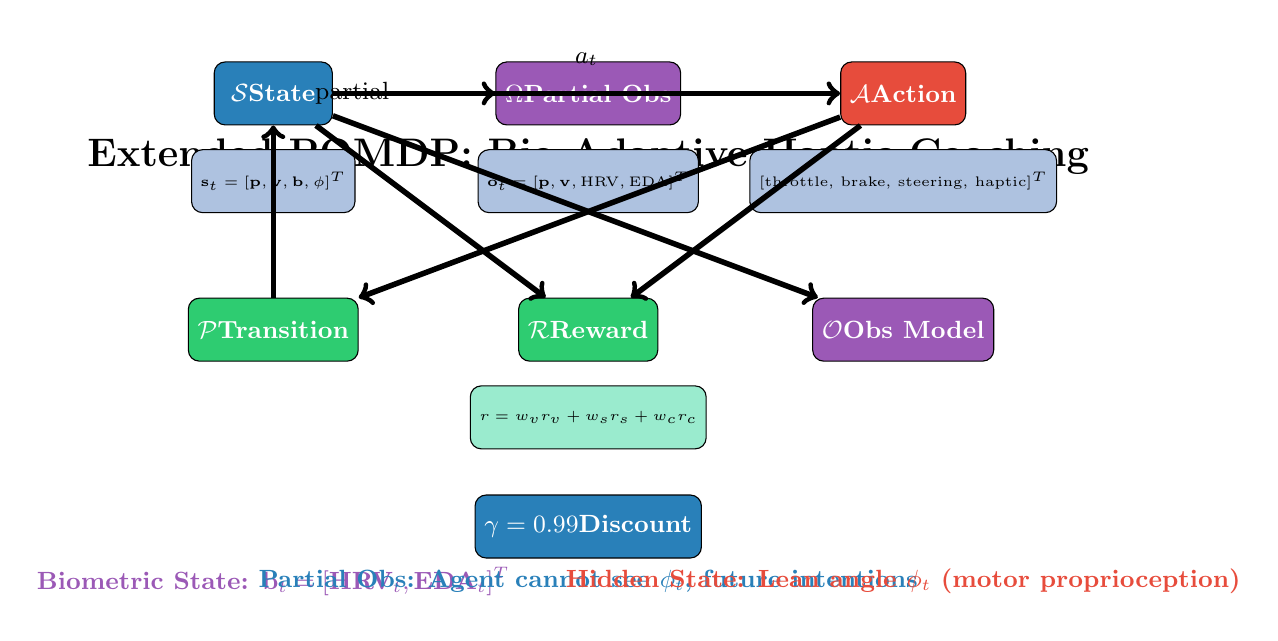
\begin{tikzpicture}[
    node distance=2.5cm,
    every node/.style={draw,rounded corners,minimum width=1.5cm,minimum height=0.8cm,font=\small\bfseries}
]

% Title
\node[draw=none,font=\Large\bfseries] at (6,-0.8) {Extended POMDP: Bio-Adaptive Haptic Coaching};

% State space
\node[fill=pomdpblue,text=white] (state) at (2,0) {$\mathcal{S}$\\State};
\node[fill=lightblue,text=black,below=0.3cm of state,draw,font=\tiny,rounded corners] {$\mathbf{s}_t = [\mathbf{p}, \mathbf{v}, \mathbf{b}, \phi]^T$};

% Observation space (partial)
\node[fill=biomarkerviolet,text=white] (obs) at (6,0) {$\Omega$\\Partial Obs};
\node[fill=lightblue,text=black,below=0.3cm of obs,draw,font=\tiny,rounded corners] {$\mathbf{o}_t = [\mathbf{p}, \mathbf{v}, \text{HRV}, \text{EDA}]^T$};

% Action space
\node[fill=hapticsred,text=white] (action) at (10,0) {$\mathcal{A}$\\Action};
\node[fill=lightblue,text=black,below=0.3cm of action,draw,font=\tiny,rounded corners] {$[\text{throttle, brake, steering, haptic}]^T$};

% Transition model
\node[fill=rewardgreen,text=white] (trans) at (2,-3) {$\mathcal{P}$\\Transition};

% Reward function
\node[fill=rewardgreen,text=white] (reward) at (6,-3) {$\mathcal{R}$\\Reward};
\node[fill=lightgreen,text=black,below=0.3cm of reward,draw,font=\tiny,rounded corners] {$r = w_v r_v + w_s r_s + w_c r_c$};

% Observation model
\node[fill=biomarkerviolet,text=white] (obsmodel) at (10,-3) {$\mathcal{O}$\\Obs Model};

% Discount factor
\node[fill=pomdpblue,text=white] (discount) at (6,-5.5) {$\gamma = 0.99$\\Discount};

% Connections
\draw[->,line width=2pt] (state) -- node[above,draw=none,font=\small] {$a_t$} (action);
\draw[->,line width=2pt] (action) -- (trans);
\draw[->,line width=2pt] (trans) -- (state);
\draw[->,line width=2pt] (state) -- (reward);
\draw[->,line width=2pt] (action) -- (reward);
\draw[->,line width=2pt] (state) -- node[left,draw=none,font=\small] {partial} (obs);
\draw[->,line width=2pt] (state) -- (obsmodel);

% Biometric component highlight
\node[draw=none,font=\small\bfseries,text=biomarkerviolet] at (2,-6.2) {\textbf{Biometric State:} $\mathbf{b}_t = [\text{HRV}_t, \text{EDA}_t]^T$};
\node[draw=none,font=\small\bfseries,text=pomdpblue] at (6,-6.2) {\textbf{Partial Obs:} Agent cannot see $\phi_t$, future intentions};
\node[draw=none,font=\small\bfseries,text=hapticsred] at (10,-6.2) {\textbf{Hidden State:} Lean angle $\phi_t$ (motor proprioception)};

\end{tikzpicture}

\pagebreak

% ============================================================================
% FIGURE 2: MULTI-OBJECTIVE REWARD SCALARIZATION
% ============================================================================

\begin{tikzpicture}

% Title
\node[draw=none,font=\Large\bfseries] at (7,-0.5) {Multi-Objective Reward Scalarization};

% Velocity reward
\begin{scope}[shift=(0,0)]
\node[fill=rewardgreen,text=white,font=\small\bfseries] at (2,2) {$r_v$ (Velocity)};
\draw[thick, rewardgreen] (0.5,0) -- (1,0.3) -- (2,0.8) -- (3,1.2) -- (3.5,1.5);
\draw[dashed,gray] (0,0) -- (4,0) -- (4,2) -- (0,2) -- (0,0);
\node[draw=none,font=\tiny] at (2,-0.4) {Speed $\rightarrow$};
\node[draw=none,font=\tiny] at (-0.5,1) {Reward};
\node[draw=none,font=\tiny] at (2,-0.8) {Weight: $w_v = 0.50$};
\end{scope}

% Safety reward
\begin{scope}[shift=(5,0)]
\node[fill=rewardgreen,text=white,font=\small\bfseries] at (2,2) {$r_s$ (Safety)};
\draw[thick, rewardgreen] (0.5,0.05) -- (1,0.3) -- (2,0.8) -- (3,1.3) -- (3.5,1.45);
\draw[dashed,gray] (0,0) -- (4,0) -- (4,2) -- (0,2) -- (0,0);
\node[draw=none,font=\tiny] at (2,-0.4) {Distance to obstacle};
\node[draw=none,font=\tiny] at (-0.5,1) {Reward};
\node[draw=none,font=\tiny] at (2,-0.8) {Weight: $w_s = 0.35$};
\end{scope}

% Cognitive Load reward
\begin{scope}[shift=(10,0)]
\node[fill=biomarkerviolet,text=white,font=\small\bfseries] at (2,2) {$r_c$ (Cog Load)};
% Safe zone
\draw[thick, biomarkerviolet] (0.5,1.5) -- (1.8,1.5);
% Risk zone
\draw[thick, biomarkerviolet] (1.8,1.5) -- (3,0.3);
% Panic zone
\draw[thick, biomarkerviolet, dashed] (3,0.3) -- (3.5,-0.5);
\draw[dashed,gray] (0,0) -- (4,0) -- (4,2) -- (0,2) -- (0,0);
\node[draw=none,font=\tiny,text=green] at (1.2,1.8) {RMSSD>50};
\node[draw=none,font=\tiny,text=orange] at (2.5,0.8) {10-50};
\node[draw=none,font=\tiny,text=red] at (3.2,-0.2) {<10};
\node[draw=none,font=\tiny] at (-0.5,1) {Reward};
\node[draw=none,font=\tiny] at (2,-0.8) {Weight: $w_c = 0.15$};
\end{scope}

% Weighted combination
\node[draw=none,font=\normalsize\bfseries,fill=yellow!20,inner sep=10pt] at (7,-2.5) {$r_t = 0.50 \cdot r_v + 0.35 \cdot r_s + 0.15 \cdot r_c$};

\node[draw=none,font=\tiny,text=darkgray,inner sep=5pt] at (7,-3.3) {Objective function: $J(\pi) = \mathbb{E}[\sum_t \gamma^t r_t]$ maximized by policy gradient};

\end{tikzpicture}

\pagebreak

% ============================================================================
% FIGURE 3: BIO-SUPERVISOR ARCHITECTURE
% ============================================================================

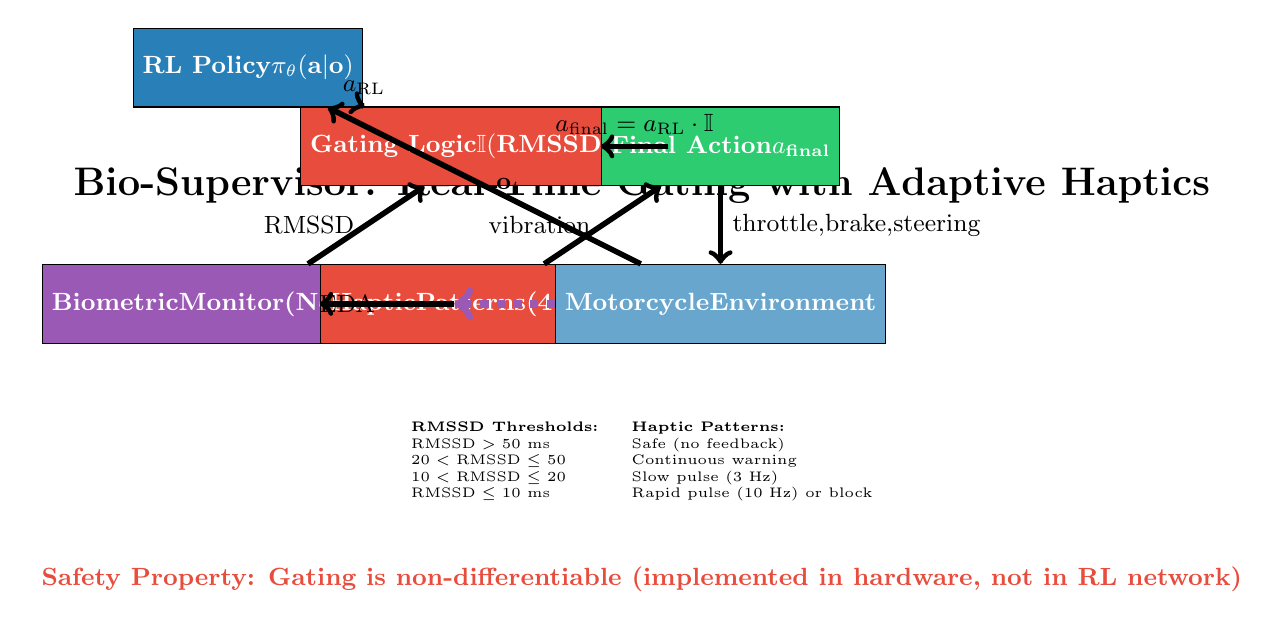
\begin{tikzpicture}[
    node distance=2cm,
]

% Title
\node[draw=none,font=\Large\bfseries] at (7,-0.5) {Bio-Supervisor: Real-Time Gating with Adaptive Haptics};

% RL Policy
\node[draw,fill=pomdpblue,text=white,font=\small\bfseries,minimum width=2.5cm,minimum height=1cm] (rl) at (2,1) {RL Policy\\$\pi_\theta(\mathbf{a}|\mathbf{o})$};

% Biometric Monitor
\node[draw,fill=biomarkerviolet,text=white,font=\small\bfseries,minimum width=2.5cm,minimum height=1cm] (bio) at (2,-2) {Biometric\\Monitor\\(NeuroKit2)};

% Gating logic
\node[draw,fill=hapticsred,text=white,font=\small\bfseries,minimum width=2.5cm,minimum height=1cm] (gating) at (5,0) {Gating Logic\\$\mathbb{I}(\text{RMSSD} > \theta)$};

% Haptic feedback
\node[draw,fill=hapticsred,text=white,font=\small\bfseries,minimum width=2.5cm,minimum height=1cm] (haptic) at (5,-2) {Haptic\\Patterns\\(4-stage)};

% Final action
\node[draw,fill=rewardgreen,text=white,font=\small\bfseries,minimum width=2.5cm,minimum height=1cm] (action) at (8,0) {Final Action\\$a_{\text{final}}$};

% Motorcycle environment
\node[draw,fill=pomdpblue!70,text=white,font=\small\bfseries,minimum width=2.5cm,minimum height=1cm] (env) at (8,-2) {Motorcycle\\Environment};

% Connections
\draw[->,line width=2pt] (rl) -- node[above,draw=none,font=\small] {$a_{\text{RL}}$} (gating);
\draw[->,line width=2pt] (gating) -- node[above,draw=none,font=\small] {$a_{\text{final}} = a_{\text{RL}} \cdot \mathbb{I}$} (action);

\draw[->,line width=2pt] (bio) -- node[left,draw=none,font=\small] {RMSSD} (gating);
\draw[->,line width=2pt] (bio) -- node[left,draw=none,font=\small] {EDA} (haptic);
\draw[->,line width=2pt] (haptic) -- node[left,draw=none,font=\small] {vibration} (action);

\draw[->,line width=2pt] (action) -- node[right,draw=none,font=\small] {throttle,\\brake,\\steering} (env);
\draw[->,line width=3pt,dashed,biomarkerviolet] (env) -- (bio);
\draw[->,line width=2pt] (env) -- node[right,draw=none,font=\small] {$\mathbf{o}_t$} (rl);

% Legend box
\node[draw=none,font=\tiny,inner sep=5pt] at (7,-4) {
\begin{tabular}{ll}
\textbf{RMSSD Thresholds:} & \textbf{Haptic Patterns:} \\
$\text{RMSSD} > 50$ ms & Safe (no feedback) \\
$20 < \text{RMSSD} \leq 50$ & Continuous warning \\
$10 < \text{RMSSD} \leq 20$ & Slow pulse (3 Hz) \\
$\text{RMSSD} \leq 10$ ms & Rapid pulse (10 Hz) or block \\
\end{tabular}
};

\node[draw=none,font=\small\bfseries,text=hapticsred,inner sep=5pt] at (7,-5.5) {\textbf{Safety Property:} Gating is non-differentiable (implemented in hardware, not in RL network)};

\end{tikzpicture}

\pagebreak

% ============================================================================
% FIGURE 4: POLICY ARCHITECTURE WITH BIOMETRIC FUSION
% ============================================================================

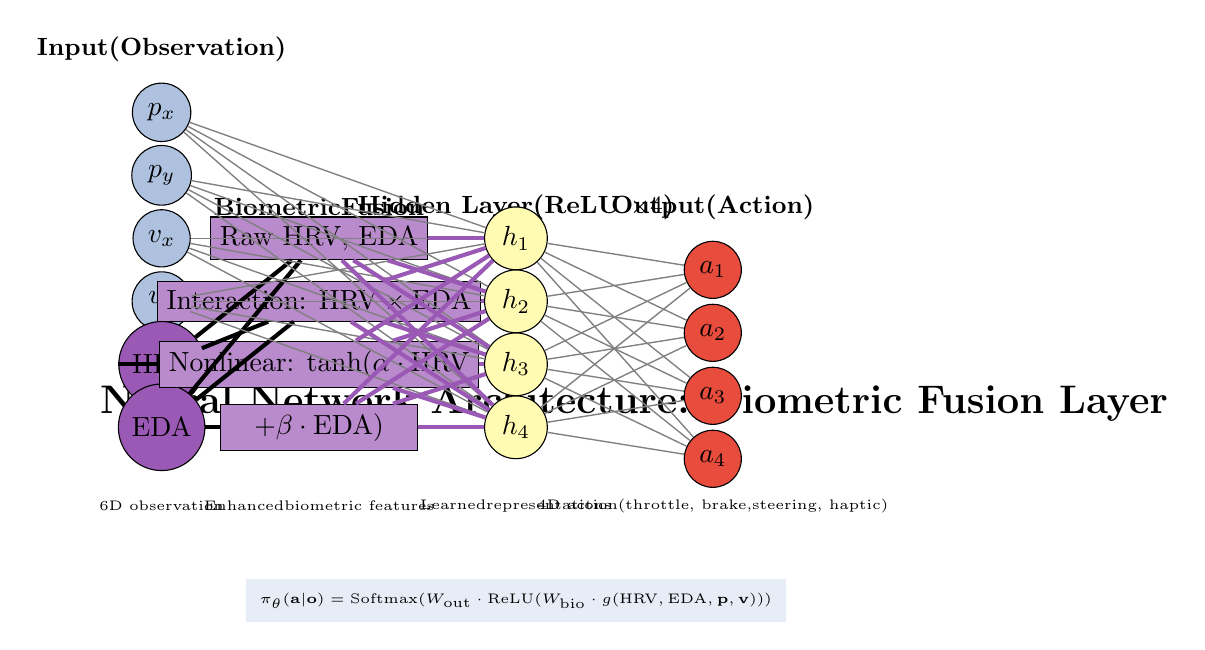
\begin{tikzpicture}[
    node distance=1.5cm,
]

% Title
\node[draw=none,font=\Large\bfseries] at (7,-0.5) {Neural Network Architecture: Biometric Fusion Layer};

% Input layer
\node[draw=none,font=\small\bfseries] at (1,4) {Input\\(Observation)};

\node[draw,fill=lightblue,circle,minimum size=0.6cm] (p1) at (1,3.2) {$p_x$};
\node[draw,fill=lightblue,circle,minimum size=0.6cm] (p2) at (1,2.4) {$p_y$};
\node[draw,fill=lightblue,circle,minimum size=0.6cm] (v1) at (1,1.6) {$v_x$};
\node[draw,fill=lightblue,circle,minimum size=0.6cm] (v2) at (1,0.8) {$v_y$};
\node[draw,fill=biomarkerviolet,circle,minimum size=0.6cm] (hrv) at (1,0) {HRV};
\node[draw,fill=biomarkerviolet,circle,minimum size=0.6cm] (eda) at (1,-0.8) {EDA};

% Biometric fusion layer
\node[draw=none,font=\small\bfseries] at (3,2) {Biometric\\Fusion};

\node[draw,fill=biomarkerviolet!70,rectangle,minimum width=2.5cm,minimum height=0.5cm] (fusion1) at (3,1.6) {Raw HRV, EDA};
\node[draw,fill=biomarkerviolet!70,rectangle,minimum width=2.5cm,minimum height=0.5cm] (fusion2) at (3,0.8) {Interaction: $\text{HRV} \times \text{EDA}$};
\node[draw,fill=biomarkerviolet!70,rectangle,minimum width=2.5cm,minimum height=0.5cm] (fusion3) at (3,0) {Nonlinear: $\tanh(\alpha\cdot\text{HRV}$};
\node[draw,fill=biomarkerviolet!70,rectangle,minimum width=2.5cm,minimum height=0.5cm] (fusion4) at (3,-0.8) {$+\beta\cdot\text{EDA})$};

% Hidden layer
\node[draw=none,font=\small\bfseries] at (5.5,2) {Hidden Layer\\(ReLU $\times 4$)};

\node[draw,fill=yellow!30,circle,minimum size=0.6cm] (h1) at (5.5,1.6) {$h_1$};
\node[draw,fill=yellow!30,circle,minimum size=0.6cm] (h2) at (5.5,0.8) {$h_2$};
\node[draw,fill=yellow!30,circle,minimum size=0.6cm] (h3) at (5.5,0) {$h_3$};
\node[draw,fill=yellow!30,circle,minimum size=0.6cm] (h4) at (5.5,-0.8) {$h_4$};

% Output layer
\node[draw=none,font=\small\bfseries] at (8,2) {Output\\(Action)};

\node[draw,fill=hapticsred,circle,minimum size=0.6cm] (a1) at (8,1.2) {$a_1$};
\node[draw,fill=hapticsred,circle,minimum size=0.6cm] (a2) at (8,0.4) {$a_2$};
\node[draw,fill=hapticsred,circle,minimum size=0.6cm] (a3) at (8,-0.4) {$a_3$};
\node[draw,fill=hapticsred,circle,minimum size=0.6cm] (a4) at (8,-1.2) {$a_4$};

% Connections from input to fusion
\draw[-,line width=1.5pt] (hrv) -- (fusion1);
\draw[-,line width=1.5pt] (eda) -- (fusion1);
\draw[-,line width=1.5pt] (hrv) -- (fusion2);
\draw[-,line width=1.5pt] (eda) -- (fusion2);
\draw[-,line width=1.5pt] (hrv) -- (fusion3);
\draw[-,line width=1.5pt] (eda) -- (fusion4);

% Connections from position/velocity to hidden
\foreach \s in {p1,p2,v1,v2}
    \foreach \h in {h1,h2,h3,h4}
        \draw[-,line width=0.5pt,gray] (\s) -- (\h);

% Connections from fusion to hidden
\foreach \f in {fusion1,fusion2,fusion3,fusion4}
    \foreach \h in {h1,h2,h3,h4}
        \draw[-,line width=1.5pt,biomarkerviolet] (\f) -- (\h);

% Connections from hidden to output
\foreach \h in {h1,h2,h3,h4}
    \foreach \a in {a1,a2,a3,a4}
        \draw[-,line width=0.5pt,gray] (\h) -- (\a);

% Labels
\node[draw=none,font=\tiny] at (1,-1.8) {6D observation};
\node[draw=none,font=\tiny] at (3,-1.8) {Enhanced\\biometric features};
\node[draw=none,font=\tiny] at (5.5,-1.8) {Learned\\representations};
\node[draw=none,font=\tiny] at (8,-1.8) {4D action\\(throttle, brake,\\steering, haptic)};

% Formula box
\node[draw=none,font=\tiny,inner sep=5pt,fill=lightblue!30] at (5.5,-3) {
$\pi_\theta(\mathbf{a}|\mathbf{o}) = \text{Softmax}(W_{\text{out}} \cdot \text{ReLU}(W_{\text{bio}} \cdot g(\text{HRV}, \text{EDA}, \mathbf{p}, \mathbf{v})))$
};

\end{tikzpicture}

\pagebreak

% ============================================================================
% FIGURE 5: RMSSD-BASED COGNITIVE LOAD REWARD
% ============================================================================

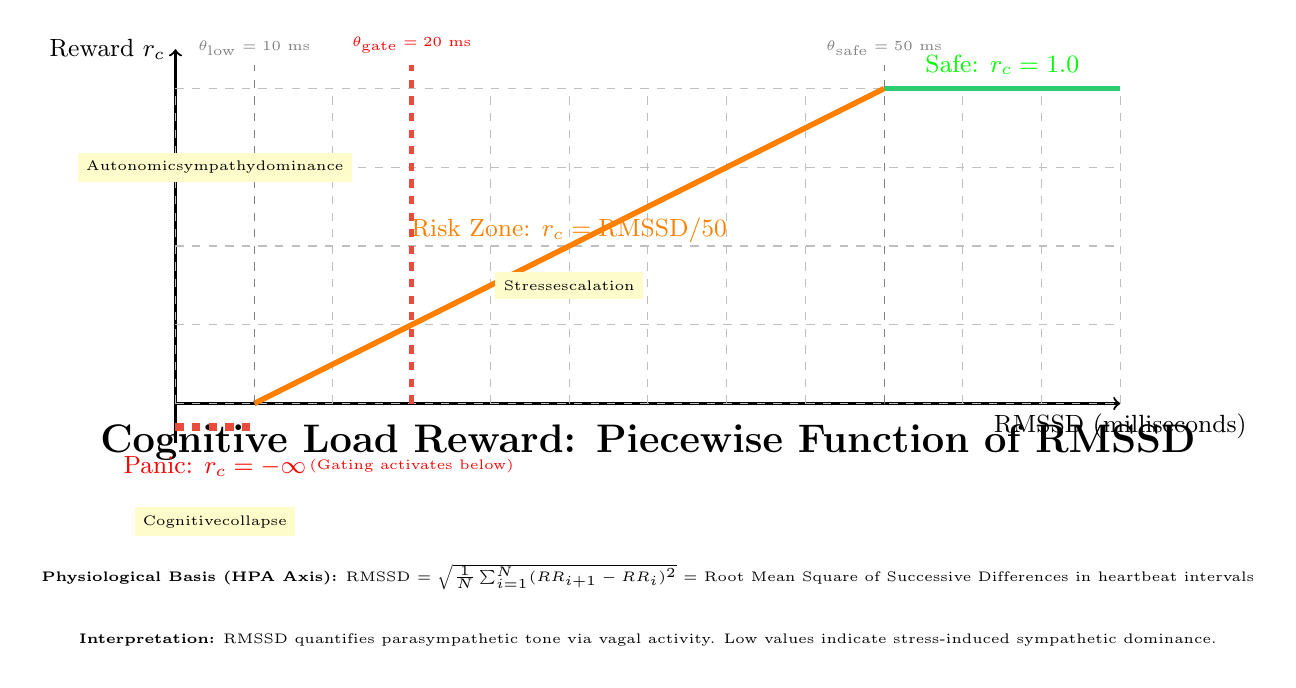
\begin{tikzpicture}

% Title
\node[draw=none,font=\Large\bfseries] at (7,-0.5) {Cognitive Load Reward: Piecewise Function of RMSSD};

% Axes
\draw[thick,->] (1,0) -- (13,0) node[below,font=\small] {RMSSD (milliseconds)};
\draw[thick,->] (1,-0.5) -- (1,4.5) node[left,font=\small] {Reward $r_c$};

% Grid
\draw[dashed,gray!50] (1,0) grid[step=1] (13,4);

% Function pieces
% Safe zone (RMSSD >= 50)
\draw[thick, rewardgreen, line width=2pt] (10,4) -- (13,4);
\node[draw=none,font=\small,text=green] at (11.5,4.3) {Safe: $r_c = 1.0$};

% Linear zone (10 < RMSSD < 50)
\draw[thick, orange, line width=2pt] (2,0) -- (10,4);
\node[draw=none,font=\small,text=orange] at (6,2.2) {Risk Zone: $r_c = \text{RMSSD}/50$};

% Panic zone (RMSSD <= 10)
\draw[thick, hapticsred, line width=3pt, dashed] (1,-0.3) -- (2,-0.3);
\node[draw=none,font=\small,text=red] at (1.5,-0.8) {Panic: $r_c = -\infty$};

% Threshold lines
\draw[dashed, gray] (2,0) -- (2,4.3) node[above,font=\tiny] {$\theta_{\text{low}} = 10$ ms};
\draw[dashed, gray] (10,0) -- (10,4.3) node[above,font=\tiny] {$\theta_{\text{safe}} = 50$ ms};

% Gating threshold
\draw[dashed, hapticsred, line width=2pt] (4,0) -- (4,4.3) node[above,font=\tiny,text=red] {$\theta_{\text{gate}} = 20$ ms};
\node[draw=none,font=\tiny,text=red] at (4,-0.8) {(Gating activates below)};

% Annotations
\node[draw=none,font=\tiny,inner sep=3pt,fill=yellow!20] at (1.5,3) {Autonomic\\sympathy\\dominance};
\node[draw=none,font=\tiny,inner sep=3pt,fill=yellow!20] at (6,1.5) {Stress\\escalation};
\node[draw=none,font=\tiny,inner sep=3pt,fill=yellow!20] at (1.5,-1.5) {Cognitive\\collapse};

% Legend
\node[draw=none,font=\tiny,inner sep=5pt] at (7,-2.2) {
\textbf{Physiological Basis (HPA Axis):}
RMSSD = $\sqrt{\frac{1}{N}\sum_{i=1}^N (RR_{i+1} - RR_i)^2}$ = Root Mean Square of Successive Differences in heartbeat intervals
};

\node[draw=none,font=\tiny,inner sep=5pt] at (7,-3) {
\textbf{Interpretation:} RMSSD quantifies parasympathetic tone via vagal activity. Low values indicate stress-induced sympathetic dominance.
};

\end{tikzpicture}

\pagebreak

% ============================================================================
% FIGURE 6: STATE SPACE DIMENSIONALITY
% ============================================================================

\begin{tikzpicture}

% Title
\node[draw=none,font=\Large\bfseries] at (7,-0.5) {State Space: 7D Hidden vs 6D Observed};

% Hidden state box
\node[draw,fill=pomdpblue,text=white,font=\small\bfseries,minimum width=4cm,minimum height=3cm] (hidden) at (2.5,1.5) {
\begin{tabular}{c}
\textbf{Hidden State} $\mathbf{s}_t \in \mathbb{R}^7$ \\
\\
$p_x$ (position X) \\
$p_y$ (position Y) \\
$v_x$ (velocity X) \\
$v_y$ (velocity Y) \\
HRV (Heart Rate Var.) \\
EDA (Electro. Dermal) \\
$\phi$ (lean angle) \textcolor{red}{???}
\end{tabular}
};

% Observation box
\node[draw,fill=biomarkerviolet,text=white,font=\small\bfseries,minimum width=4cm,minimum height=2.5cm] (obs) at (7.5,1.5) {
\begin{tabular}{c}
\textbf{Observed} $\mathbf{o}_t \in \mathbb{R}^6$ \\
\\
$p_x$ (position X) \\
$p_y$ (position Y) \\
$v_x$ (velocity X) \\
$v_y$ (velocity Y) \\
HRV (Heart Rate Var.) \\
EDA (Electro. Dermal)
\end{tabular}
};

% Arrow showing loss of information
\draw[->,line width=3pt,red] (4.8,2) -- (5.7,2) node[above,draw=none,font=\small,text=red] {Partial\\Observability};

% Explanation
\node[draw=none,font=\small,text=darkred,inner sep=5pt,fill=red!10] at (5,0.3) {
Motorcycle lean angle $\phi$ is \textbf{hidden} from agent \\
(proprioceptive sensing not available in coaching context)
};

% Agent belief
\node[draw,fill=rewardgreen!70,text=white,font=\small\bfseries,minimum width=3cm,minimum height=1.5cm] (belief) at (5,-2.5) {
\begin{tabular}{c}
\textbf{Agent Belief} \\
State via Bayesian Filter \\
$b_t(s_t) = \frac{\mathcal{O}(o_t|s_t) P(s_t|s_{t-1},a_{t-1}) b_{t-1}(s_{t-1})}{\mathcal{O}(o_t)}$
\end{tabular}
};

\draw[->,line width=2pt] (2.5,0.2) -- (belief);
\draw[->,line width=2pt] (7.5,0.2) -- (belief);

\end{tikzpicture}

\pagebreak

% ============================================================================
% FIGURE 7: TRAINING ALGORITHM FLOWCHART
% ============================================================================

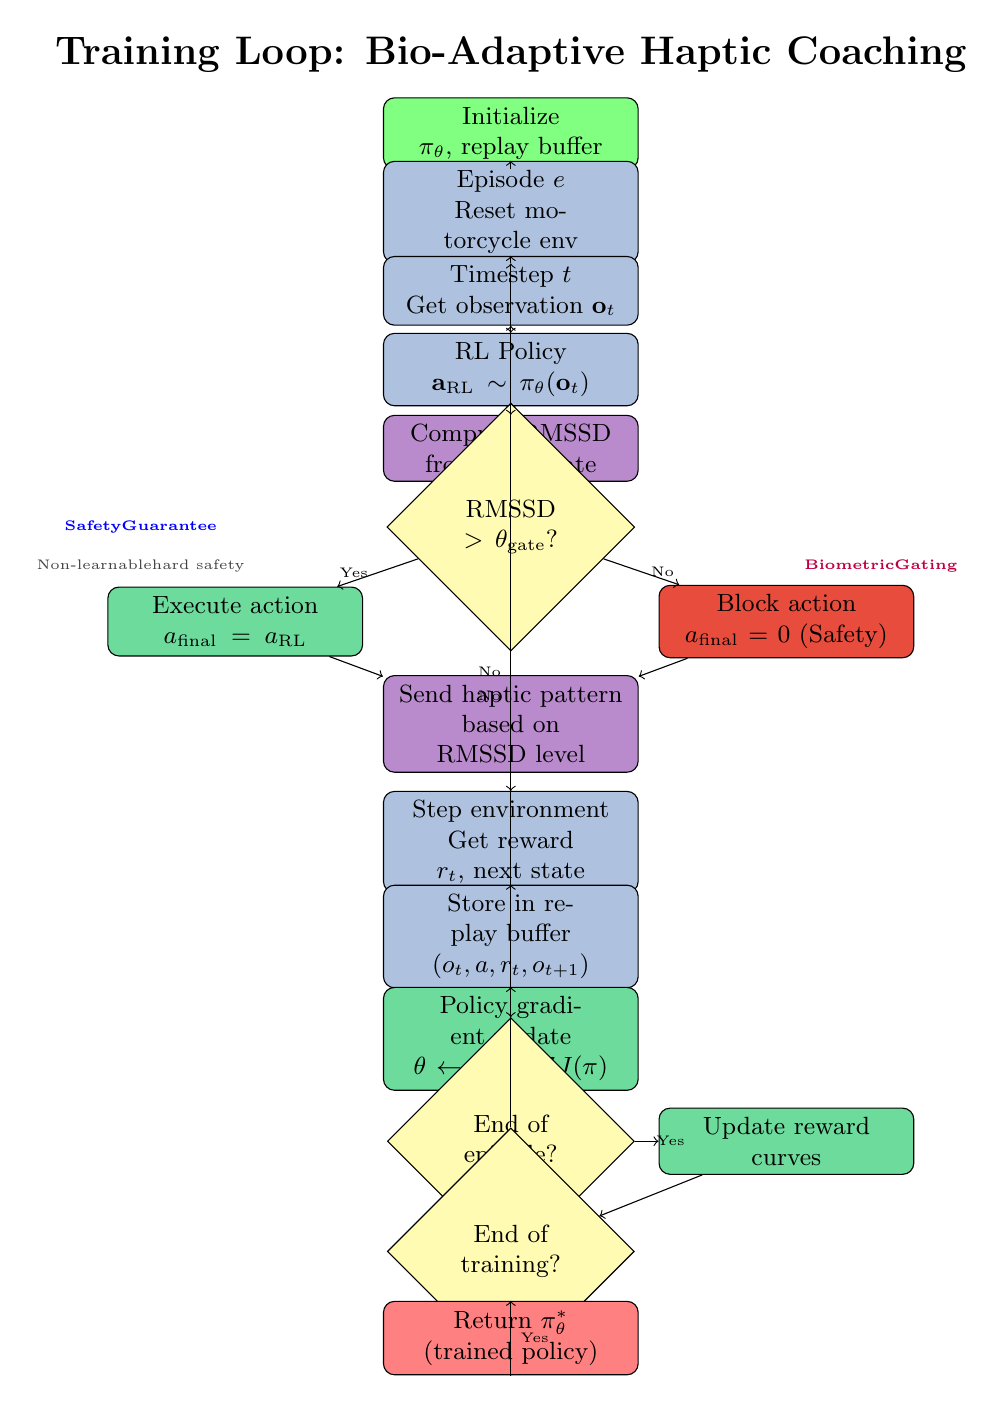
\begin{tikzpicture}[
    node distance=1.8cm,
    block/.style={draw, fill=lightblue, text width=3cm, text centered, rounded corners, minimum height=0.8cm, font=\small},
    decision/.style={diamond, draw, fill=yellow!30, text width=2cm, text centered, minimum height=1cm, font=\small},
    action/.style={draw, fill=rewardgreen!70, text width=3cm, text centered, rounded corners, minimum height=0.8cm, font=\small},
    bioaction/.style={draw, fill=biomarkerviolet!70, text width=3cm, text centered, rounded corners, minimum height=0.8cm, font=\small}
]

% Title
\node[draw=none,font=\Large\bfseries] at (5,9) {Training Loop: Bio-Adaptive Haptic Coaching};

% Start
\node[block,fill=green!50] (start) at (5,8) {Initialize\\$\pi_\theta$, replay buffer};

% Episode
\node[block] (episode) at (5,7) {Episode $e$\\Reset motorcycle env};

% Timestep
\node[block] (timestep) at (5,6) {Timestep $t$\\Get observation $\mathbf{o}_t$};

% Action selection
\node[block] (action) at (5,5) {RL Policy\\$\mathbf{a}_{\text{RL}} \sim \pi_\theta(\mathbf{o}_t)$};

% Compute RMSSD
\node[bioaction] (rmssd) at (5,4) {Compute RMSSD\\from heart rate};

% Gating decision
\node[decision] (gate) at (5,3) {RMSSD\\$> \theta_{\text{gate}}$?};

% Gating true
\node[action] (gate_true) at (1.5,1.8) {Execute action\\$a_{\text{final}} = a_{\text{RL}}$};

% Gating false
\node[action,fill=hapticsred] (gate_false) at (8.5,1.8) {Block action\\$a_{\text{final}} = 0$ (Safety)};

% Haptic feedback
\node[bioaction] (haptic) at (5,0.5) {Send haptic pattern\\based on RMSSD level};

% Step environment
\node[block] (step) at (5,-1) {Step environment\\Get reward $r_t$, next state};

% Store transition
\node[block] (store) at (5,-2.2) {Store in replay buffer\\$(o_t, a, r_t, o_{t+1})$};

% Update policy
\node[action] (update) at (5,-3.5) {Policy gradient update\\$\theta \leftarrow \theta + \alpha \nabla J(\pi)$};

% End of episode?
\node[decision] (eod) at (5,-4.8) {End of\\episode?};

% Update curves
\node[action] (curves) at (8.5,-4.8) {Update reward\\curves};

% End training?
\node[decision] (eot) at (5,-6.2) {End of\\training?};

% End
\node[block,fill=red!50] (end) at (5,-7.3) {Return $\pi_\theta^*$\\(trained policy)};

% Connections
\draw[->] (start) -- (episode);
\draw[->] (episode) -- (timestep);
\draw[->] (timestep) -- (action);
\draw[->] (action) -- (rmssd);
\draw[->] (rmssd) -- (gate);

\draw[->] (gate) -- node[left,draw=none,font=\tiny] {Yes} (gate_true);
\draw[->] (gate) -- node[right,draw=none,font=\tiny] {No} (gate_false);

\draw[->] (gate_true) -- (haptic);
\draw[->] (gate_false) -- (haptic);

\draw[->] (haptic) -- (step);
\draw[->] (step) -- (store);
\draw[->] (store) -- (update);

\draw[->] (update) -- (eod);
\draw[->] (eod) -- node[left,draw=none,font=\tiny] {No} (timestep);
\draw[->] (eod) -- node[right,draw=none,font=\tiny] {Yes} (curves);

\draw[->] (curves) -- (eot);
\draw[->] (eot) -- node[left,draw=none,font=\tiny] {No} (episode);
\draw[->] (eot) -- node[right,draw=none,font=\tiny] {Yes} (end);

% Side notes
\node[draw=none,font=\tiny,text=blue,inner sep=3pt] at (0.3,3) {\textbf{Safety\\Guarantee}};
\node[draw=none,font=\tiny,text=darkgray] at (0.3,2.5) {Non-learnable\\hard safety};

\node[draw=none,font=\tiny,text=purple,inner sep=3pt] at (9.7,2.5) {\textbf{Biometric\\Gating}};

\end{tikzpicture}

\end{document}
